% CVPR 2022 Paper Template
% based on the CVPR template provided by Ming-Ming Cheng (https://github.com/MCG-NKU/CVPR_Template)
% modified and extended by Stefan Roth (stefan.roth@NOSPAMtu-darmstadt.de)

\documentclass[10pt,twocolumn,letterpaper]{article}

%%%%%%%%% PAPER TYPE  - PLEASE UPDATE FOR FINAL VERSION
% \usepackage[review]{cvpr}      % To produce the REVIEW version
% \usepackage{cvpr}              % To produce the CAMERA-READY version
\usepackage[pagenumbers]{cvpr} % To force page numbers, e.g. for an arXiv version

% Include other packages here, before hyperref.
\usepackage{graphicx}
\usepackage{amsmath}
\usepackage{amssymb}
\usepackage{booktabs}
\usepackage{multicol}
\usepackage{multirow}
\usepackage{makecell}
\usepackage{algorithm}
\usepackage{algpseudocode}
\usepackage[table]{xcolor}
\usepackage{comment}
\usepackage{tabularx}

% \usepackage[accsupp]{axessibility}  % Improves PDF readability for those with disabilities.

\def\mathbi#1{\textbf{\em #1}}
\DeclareMathOperator*{\argmax}{arg\,max}
\DeclareMathOperator*{\argmin}{arg\,min}

% It is strongly recommended to use hyperref, especially for the review version.
% hyperref with option pagebackref eases the reviewers' job.
% Please disable hyperref *only* if you encounter grave issues, e.g. with the
% file validation for the camera-ready version.
%
% If you comment hyperref and then uncomment it, you should delete
% ReviewTempalte.aux before re-running LaTeX.
% (Or just hit 'q' on the first LaTeX run, let it finish, and you
%  should be clear).
\usepackage[pagebackref,breaklinks,colorlinks]{hyperref}


% Support for easy cross-referencing
\usepackage[capitalize]{cleveref}
\crefname{section}{Sec.}{Secs.}
\Crefname{section}{Section}{Sections}
\Crefname{table}{Table}{Tables}
\crefname{table}{Tab.}{Tabs.}

\algblockdefx{FORALLP}{ENDFAP}[1]%
  {\textbf{for all }#1 \textbf{do in parallel}}%
  {\textbf{end for}}
\algblockdefx{FUNCDO}{ENDFUNCDO}[1]%
  {#1 \textbf{do}}%
  {\textbf{end}}
\DeclareMathAlphabet\mathbfcal{OMS}{cmsy}{b}{n}

%%%%%%%%% PAPER ID  - PLEASE UPDATE
\def\cvprPaperID{***} % *** Enter the CVPR Paper ID here
\def\confName{CVPR}
\def\confYear{2022}


\begin{document}

%%%%%%%%% TITLE - PLEASE UPDATE
\title{MeMOT: Multi-Object Tracking with Memory}

\author{
    Jiarui Cai$^1$\thanks{The work was done during an Amazon internship.} \hspace{0.35cm} Mingze Xu$^2$\thanks{Corresponding Author.} \hspace{0.25cm} Wei Li$^2$ \hspace{0.25cm} Yuanjun Xiong$^2$ \hspace{0.25cm} Wei Xia$^2$ \hspace{0.25cm} Zhuowen Tu$^2$ \hspace{0.25cm} Stefano Soatto$^2$ \\ [.5ex] $^1$University of Washington \hspace{0.9cm} $^2$AWS AI Labs \\ [.5ex]
    {\tt\small jrcai@uw.edu, \{xumingze,wayl,yuanjx,wxia,ztu,soattos\}@amazon.com}
}

\maketitle

%%%%%%%%% ABSTRACT
\begin{abstract}
    We propose an online tracking algorithm that performs the object detection and data association under a common framework, capable of linking objects after a long time span. This is realized by preserving a large spatio-temporal memory to store the identity embeddings of the tracked objects, and by adaptively referencing and aggregating useful information from the memory as needed. Our model, called MeMOT, consists of three main modules that are all Transformer-based: 1) Hypothesis Generation that produce object proposals in the current video frame; 2) Memory Encoding that extracts the core information from the memory for each tracked object; and 3) Memory Decoding that solves the object detection and data association tasks simultaneously for multi-object tracking. When evaluated on widely adopted MOT benchmark datasets, MeMOT observes very competitive performance.
\end{abstract}

%%%%%%%%% BODY TEXT
\section{Introduction}\label{sec:introduction}

From immersive communications, games, virtual production, to virtual try-on and virtual fitting rooms, having an accurate 3D presentation of the body of a person is fundamental. For this, one would typically need to use a professional 3D capture stage with many cameras pointing at the person in the center of the stage, and then put all the videos together using a 3D reconstruction algorithm, such as the ones proposed by \cite{guo2019relightables}, \cite{collet2015high} or \cite{pages2018affordable}. These setups are complex (huge amount of data to manage, complicated calibration processes, high processing times) and expensive (a high number of cameras, professional lighting, computers, GPUs, networks and more), so to overcome these challenges, modern deep learning techniques aim to simplify the capture process by replacing the multi-camera setup with a single camera, from a single viewpoint. For example, \cite{saito2019pifu}, \cite{saito2020pifuhd}, and \cite{xiu2022icon} generate a full body 3D model of a person, \cite{escribano2022texture} propose a way to generate the textures of occluded areas. However, all these techniques output relatively low-resolution considering the target application, and they struggle with complicated poses where depth is difficult to convey from a single viewpoint.

To overcome these challenges, some approaches include additional information into the capturing process, including depth, which typically comes from a consumer-level depth sensor. Although new generation consumer-level depth sensors have significantly improved during the last few years, they still present high levels of noise and sometimes fail to capture details when the subjects are at a distance where their body can be fully captured (at around 2m and farther), and they are still sensitive to sun light (which interferes with the infra-red light these sensors typically use), dark materials (which absorb infra-red light) and non-Lambertian surfaces. 

In this work, we propose a new approach to generate high-resolution depth maps of humans using a single low-resolution image as input, using denoising diffusion probabilistic models (DDPMs). Our multi-modal DDPM was trained using high-resolution depth maps, extracted from a large dataset of photorealistic 3D models captured by Volograms \citep{volograms2021}, which allows us to obtain depth maps with higher accuracy than consumer-level depth sensors.

% Featured Image
\begin{figure}[t]
  \centering
  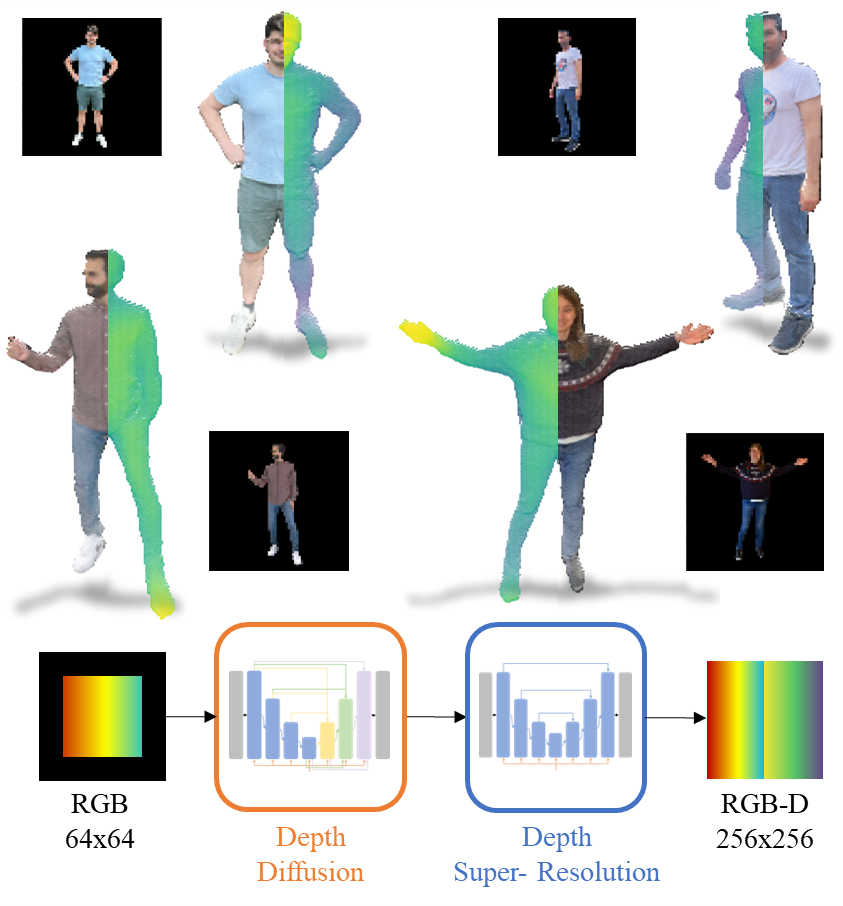
\includegraphics[width=0.99\linewidth]{illustrations/featured_image.png}
  \caption{Our \modelname{} framework generates a high-resolution RGB-D image from a low-resolution RGB image of humanoid subjects. First, a low resolution depth map is generated using a conditional DDPM. Then, the depth is upsampled to a higher resolution using a second DDPM.}
  \label{fig:featured_image}
\end{figure}

Following the taxonomy for multi-modal deep learning systems by \cite{zhan_multimodal_2022} we frame \modelname{} as a multi-modal generative translation task using a joint data representation of our input modalities RGB and depth. No alignment is performed between these modalities since our data is perfectly aligned during generation. We further perform parallel data co-learning since our RGB and depth pairs inherently share a direct correspondence between their instances.

We summarize our main contributions of this paper as follows:
\begin{enumerate}
  \item We provide a framework for high resolution dense monocular depth estimation using diffusion models.
  \item We perform super-resolution for dense depth data conditioned on a multi-modal RGB-D input condition using diffusion models. 
  \item We introduce a novel augmentation technique, namely depth noise, to enhance the robustness of the depth super-resolution model.
  \item We perform rigorous ablations and experiments to validate our design choices.
\end{enumerate}

\section{Related Work}
\label{sec:related_work}

\begin{figure*}[t!]
    \centering
    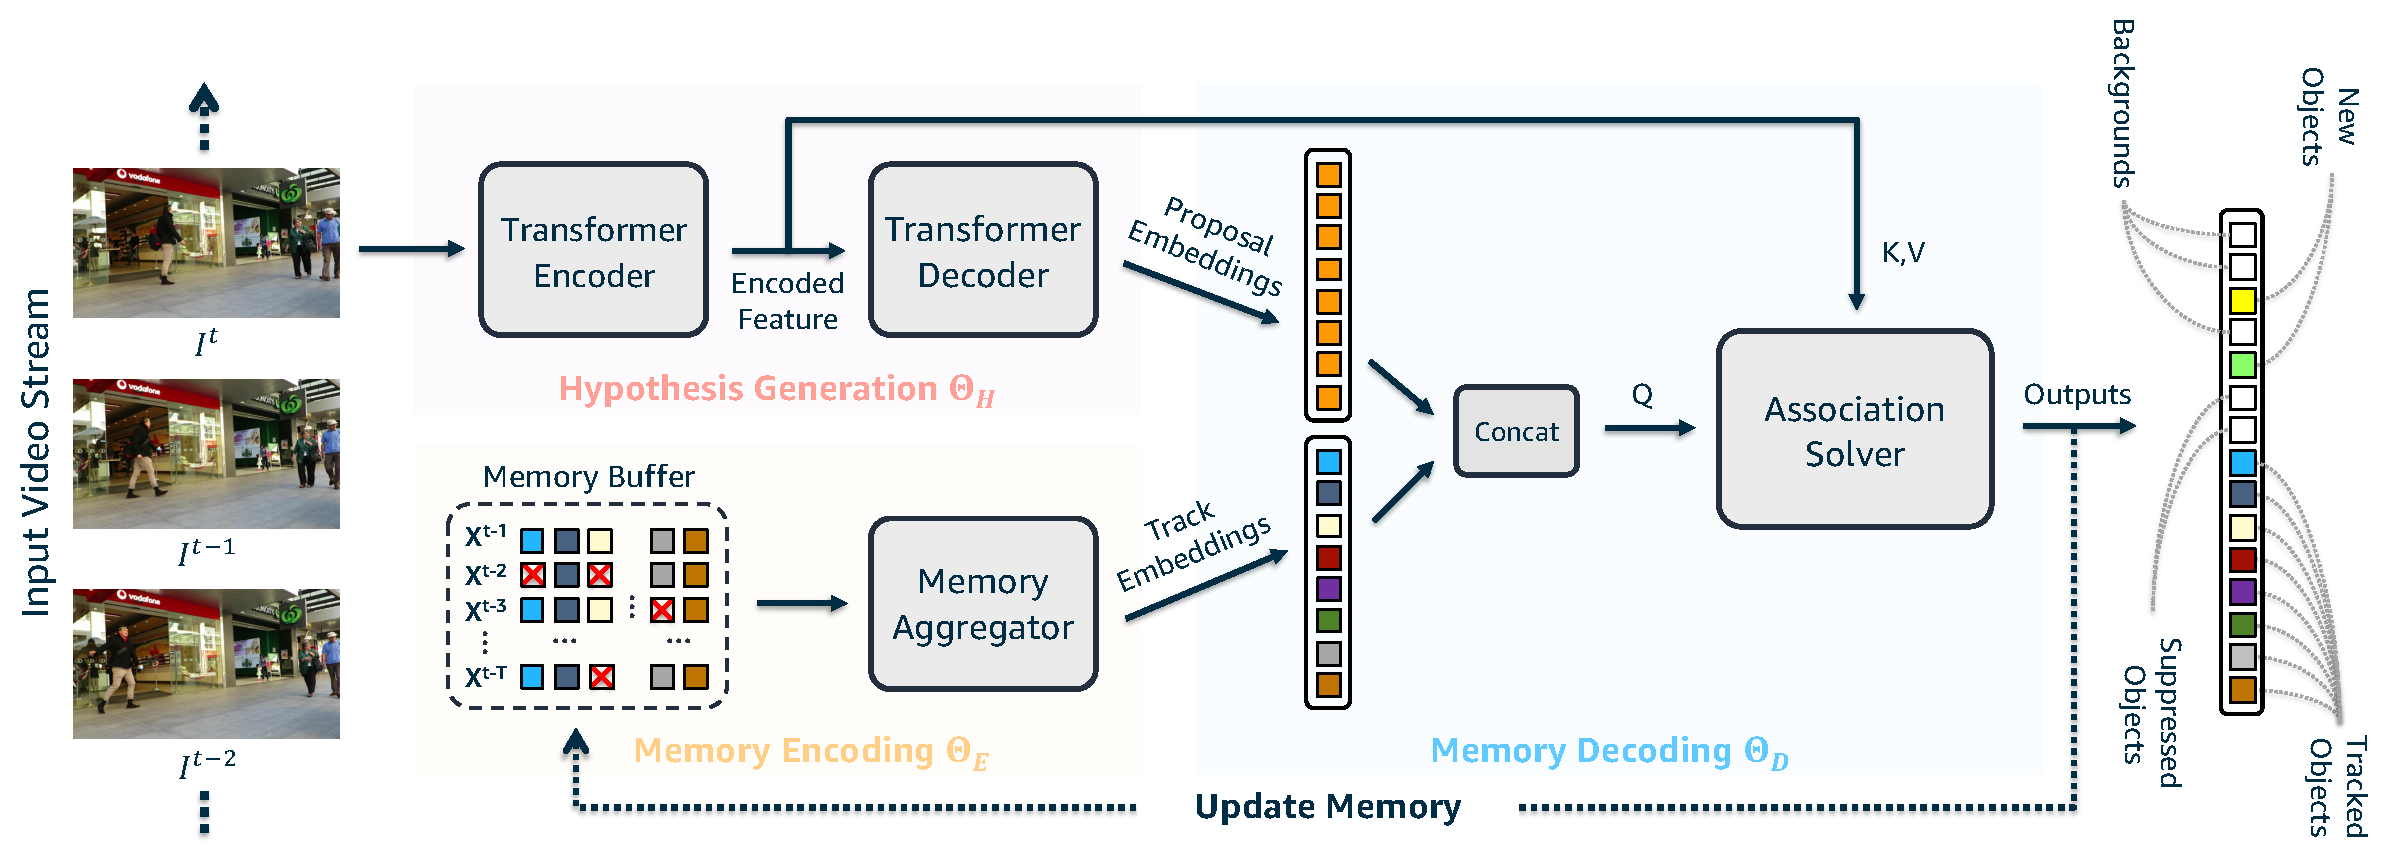
\includegraphics[width=0.97\textwidth]{figures/network.pdf}
    \vspace{-3.5mm}
    \caption{
        \textbf{Visualization of MeMOT}, which runs three main components: 1) a hypothesis generation module $\Theta_H$ that produces object proposals for the current video frame, 2) a memory encoding module $\Theta_E$ that retrieves core information for each tracked objects, and 3) a memory decoding module $\Theta_D$ that solves the object detection and data association tasks simultaneously.
        MeMOT maintains a memory buffer to store long-range states of tracked objects, together with an efficient encoding-decoding process that retrieves useful information for linking objects after a long time span.
        Each hypothetical object is predicted as a new object, a tracked object, or a background region.
    }
    \label{fig:network}
\end{figure*}

\noindent \textbf{Classical Tracking Methods}.
Tracking is well studied in computer vision~\cite{isard1998condensation,babenko2010robust,wu2013online,kristan2015visual}.
Coping with the underlying uncertainties of the tracking results~\cite{isard1998condensation} and object appearances/positions/shapes~\cite{babenko2010robust} has been a central challenge.
Classical non-deep learning methods~\cite{wu2013online} have laid out solid mathematical and statistical foundations.
Specifically, Kalman~\cite{welch1995introduction} and particle filters ~\cite{gustafsson2002particle} are widely adopted for tackling tracking problems~\cite{shen2003probabilistic,hue2001particle,xing2009multi}. The progressive observation-based Bayesian inference method~\cite{xing2010multiple} is proposed for MOT in online sports videos. A spatial and temporal shape representation-based Bayesian framework~\cite{giebel2004bayesian} is proposed for multi-cue 3D deformable object tracking. In these methods,
an optimal filter maintains tracking states that summarize history information and estimate new frame's tracking results. In a linear-Gaussian case, the optimal state can indeed be estimated, while for more general non-linear, non-Gaussian cases, it is difficult to estimate the optimal state with a finite-dimensional state representation. For instance, occlusion in visual multiple object tracking is clearly non-linear and non-Gaussian.
To tackle this challenge, tracking methods~\cite{choi2010multiple,perera2006multi} that can access multiple frames states (offline tracking) is desired.

\vspace{2pt} \noindent \textbf{MOT with CNNs}.
A typical scheme for MOT~\cite{wojke2017simple,feng2019multi,wang2019exploit,chu2019famnet} is ``tracking-by-detection'', which directly uses ready-made detectors~\cite{felzenszwalb2009object,ren2015faster,liu2016ssd,zhou2019objects,ge2021yolox} and focuses on the data association.
% Recent approaches build object detection and data association in the same network.
Tracktor++~\cite{bergmann2019tracking} propagates the bounding boxes of tracked objects as region proposals to the next frame.
CenterTrack~\cite{zhou2020tracking} takes an additional point-based heatmap as input and matches objects anywhere within the receptive field.
JDE~\cite{xu2018joint,wang2019towards,zhang2020fair,li2021semi} is built with two homogeneous branches for object detection and ReID feature extraction, respectively.
Joint detection and tracking models improve the runtime, but sacrifice the tracking recovery after occlusion and cannot reconnect long-term missing objects.

\vspace{2pt} \noindent \textbf{MOT with Transformers}.
Vision Transformers have been successfully applied in image recognition~\cite{carion2020end,dosovitskiy2020image,zhu2020deformable,liu2021swin} and video analysis~\cite{arnab2021vivit,bertasius2021space,sharir2021image,liu2021video} lately.
In tracking, TrackFormer~\cite{meinhardt2021trackformer} and MOTR~\cite{zeng2021motr} simultaneously perform the object detection and association by concatenating the object and autoregressive
track queries as inputs to the Transformer decoder in the next time step.
On the other hand, TransCenter~\cite{xu2021transcenter} and TransTrack~\cite{sun2020transtrack} only use Transformers as feature extractor and recurrently pass track features to aggressively learn aggregated embedding of each object.
TransMOT~\cite{chu2021transmot} still uses CNNs as detector and feature extractor, and learns an affinity matrix with Transformers.
The above work explores the mechanism of representing object states as dynamic embeddings. However, the modeling of long-term spatio-temporal observations and adaptive feature aggregation methods are underdeveloped.

\vspace{3pt} \noindent \textbf{Memory Networks}.
Pioneering work using memory networks has been proposed in NLP~\cite{graves2014neural,weston2014memory,sukhbaatar2015end} by focusing on temporal reasoning tasks such as question answering~\cite{xiong2016dynamic,kumar2016ask} and dialogue systems~\cite{wu2019global}.
Video analysis tasks, such as action recognition~\cite{wu2019long,xu2021long}, and video object segmentation~\cite{oh2019video,lu2020video}, leverage an external memory to store and access time-indexed features in prolonged sequences, significantly improving the ability to remember the past.
Recently, memory networks have been introduced into tracking.
MemTrack~\cite{yang2018learning} reads a residual template from memory and combines it with the initial template to update the representations of targets.
STMTrack~\cite{fu2021stmtrack} guides the information retrieval with the current frame and adaptively obtains all useful information as it needs.
However, these work focuses on single object tracking (SOT), and does not need to concern about the inter-object association.
We propose to use a large spatio-temporal memory to achieve robust object association across time for MOT.

% \section{The Proposed Method}
\section{Multi-Object Tracking with Memory}
\label{sec:method}

\subsection{Overview}
\label{sec:method:overview}

Given a sequence of video frames $\mathbi{I} = \{I^0, I^1, \cdots, I^T\}$,
the goal of online MOT is to localize a set of $K$ objects while following their trajectories $\mathbfcal{T} = \{\mathcal{T}_0, \mathcal{T}_1, \cdots, \mathcal{T}_K\}$ over time by causal processing.
In this paper, we propose an end-to-end tracking algorithm, called \textit{MeMOT}, which jointly learns the object detection and association.
Different from most existing methods~\cite{bergmann2019tracking} that propagate the states of tracked objects between adjacent frames,
we build a \textit{spatio-temporal memory} that stores long-range states of all tracked objects, together with a \textit{memory encoding-decoding} process that efficiently retrieves useful information for linking objects after a long time span.

Specifically, as shown in Figure~\ref{fig:network}, MeMOT consists of three main components:
1) a frame-level hypothesis generation module $\Theta_H$ that produces region proposals for the current video frame $I^t$,
2) a track-level memory encoding module $\Theta_E$ that aggregates track embeddings,
and 3) a memory decoding module $\Theta_D$ that associates the new detections with tracked objects.
At time step $t$,
$\Theta_H$ generates $N^t_{pro}$ region proposals, represented as proposal embeddings $\mathbi{Q}_{pro}^t \in \mathbb{R}^{N^t_{pro} \times d}$ using a Transformer-based architecture.
The memory encoder $\Theta_E$ adaptively translates the ``history states'' of each track into one compact representation, denoted as track embeddings $\mathbi{Q}_{tck}^t \in \mathbb{R}^{N^t_{tck} \times d}$. 
By querying the encoded image feature with $[\mathbi{Q}_{pro}^t, \mathbi{Q}_{tck}^t]$,
the memory decoder $\Theta_D$ computes the inter-object relations and updates the embeddings as $[\widehat{\mathbi{Q}}_{pro}^t, \widehat{\mathbi{Q}}_{tck}^t]$ accordingly.
Then the locations $[\mathbi{B}_{pro}^t, \mathbi{B}_{tck}^t]$ and confidence scores  $[\mathbi{S}_{pro}^t, \mathbi{S}_{tck}^t]$ of new and tracked objects are predicted based on these output embeddings.
Finally, the locations and states of the previously tracked objects are used to update their trajectory and the memory.
The ``new-born'' objects are initialized in $\mathbfcal{T}$ and their states are added into the memory.

\subsection{Hypothesis Generation}
\label{sec:method:theta_H}

The hypothesis generation network $\Theta_H$ is built with an encoder-decoder architecture based on Transformers~\cite{carion2020end,zhu2020deformable}.
It produces a set of $N^t_{pro}$ region proposals that either initiate ``new-born'' objects for the current video frame or update tracked objects with their latest identity and position information.
The $\Theta_H$ encoder takes a sequentialized feature map $z_0^t \in \mathbb{R}^{C \times HW}$ as inputs, which is extracted by a CNN backbone from the input frame $I^t$.
Each element in $z_0^t$ is supplemented with a unique positional encoding that indicates its spatial location.
The image feature is encoded as $z_1^t \in \mathbb{R}^{d \times HW}$ using a multi-layer Transformer encoder.
The $\Theta_H$ decoder receives the encoded feature $z_1^t$ and empty object queries (represented as learnable embeddings), and produces the final set of proposal embeddings $\mathbi{Q}_{pro}^t \in \mathbb{R}^{N_{pro}^t \times d} $.
The objectness scores and bounding boxes of each proposal can be predicted from $\mathbi{Q}_{pro}^t$.

\begin{figure}
    \centering
    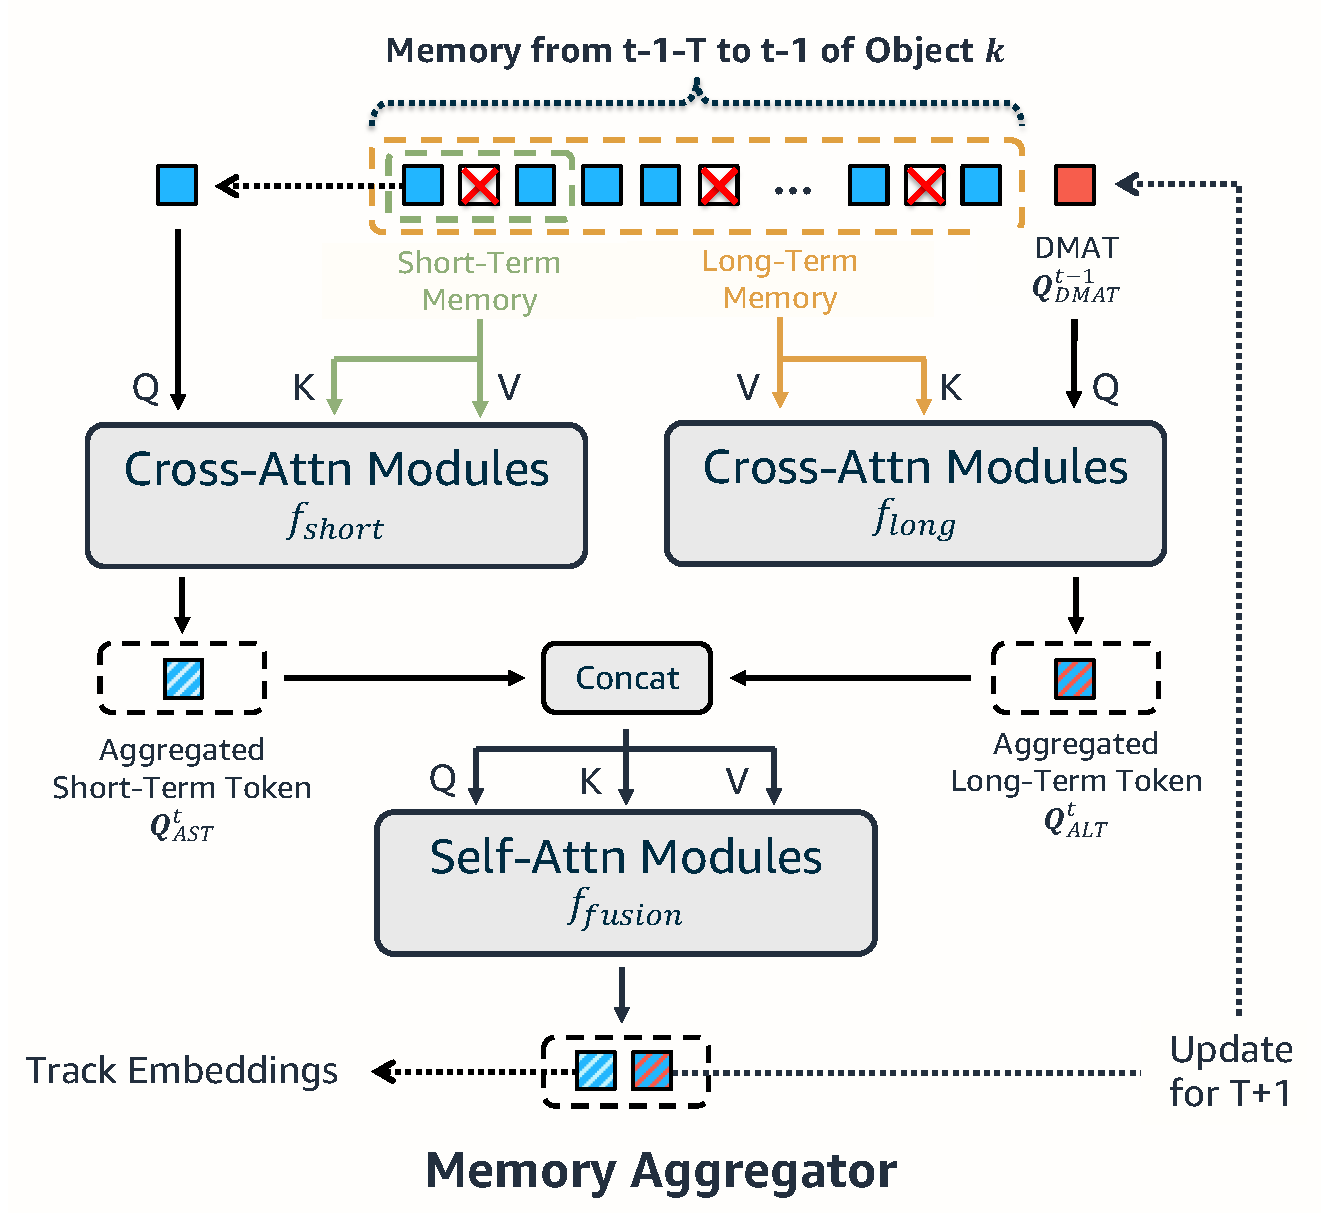
\includegraphics[width=0.5\textwidth]{figures/memory_module.pdf}
    \vspace{-7.5mm}
    \caption{
        \textbf{Illustration of Memory Aggregator}, which consists three attention modules: 1) short-term $f_{short}$ that smoothes out noises in recent frames, 2) long-term $f_{long}$ that extracts supportive features from long-range context, and 3) fusion blocks that aggregate short- and long-term branches. The aggregated embeddings will be used as the track embeddings (blue-white query) and update DMAT (blue-red query) for the next time step.
        % \textbf{Illustration of Memory Aggregator}, which consists three attention modules: 1) a short-term $f_{short}$, 2) a long-term $f_{long}$, and 3) a fusion block. The aggregated embeddings will be used as the track embeddings (blue-white query) and update DMAT (blue-red query) for the next time step.
    }
    \label{fig:ta}
    \vspace{-4.5mm}
\end{figure}

\subsection{Spatio-Temporal Memory}
\label{sec:method:memory}

We store the history states of all $N$ tracked objects in a spatio-temporal memory buffer $\mathbi{X} \in \mathbb{R}^{N \times T \times d}$.
It reserves at most $N_{max}$ objects and a maximum of $T_{max}$ time steps for each object.
The memory is implemented with a first-in-first-out (FIFO) data structure. 
At time step $t$, the memory is represented as the states of $N_{tck}^{t-1}$ active objects in the past $T$ frames, $\mathbi{X}^{t-1-T:t-1}=\{x_k^{t-1-T:t-1}\}_{k=1:N_{tck}^{t-1}}$, where $x_k^{t-1-T:t-1}$ is the states of the $k$-th object and is padded with $\mathbi{0}$ if this object does not appear in the frame $I^t$.
When $T$ is larger than $T_{max}$, the ``oldest'' state $x_k^{t-1-T}$ of each tracklet graduates from the memory.
$N_{max}$ is set to be significantly large (\eg, 300 or 600) to cover the typical number of objects in a video, and a choice of $T_{max}$ is 24.

\subsection{Memory Encoding}
\label{sec:method:theta_E}

As shown in Fig.~\ref{fig:ta}, we encode the memory and extract the track embedding with three attention modules:
1) a short-term block $f_{short}$ for assembling embeddings of neighboring frames to smooth out the noises,
2) a long-term block $f_{long}$ for extracting relevant features in the temporal window covered by the memory,
and 3) a fusion block $f_{fusion}$ for aggregating embeddings from short- and long-term branches.

For each tracklet, the short-term module $f_{short}$ takes as inputs its previous $T_s$ states while the long-term memory module $f_{long}$ utilizes longer history with length of $T_l$ ($T_s \ll T_l$).
$f_{short}$ and $f_{long}$ are implemented with multi-head cross-attention modules, where the history states are key and value inputs.
% We assume that the observations in the current frame are closer to those in the nearby frames and the long-term memory contains more redundant but supportive information.
The input query for $f_{short}$ is the most recent state $\mathbi{X}^{t-1}$, while an dynamically updated embedding, called \textit{Dynamic Memory Aggregation Tokens (DMAT)}, $\mathbi{Q}^{t-1}_{dmat} = \{{q_{dmat}}_k^{t-1}\}_{k=1:N_{tck}}$ is used for $f_{long}$.
When every tracklet is initiated, it is associated with the same DMAT as others; after that, at time step $t > 0$, DMAT is iteratively updated from the previous step. This design will be further validated in Sec.~\ref{sec:exp:ablation}.
The outputs of the short- and long-term branches, denoted as \textit{Aggregated Short-term Token (AST)} $\mathbi{Q}^t_{AST}$ and \textit{Aggregated Long-term Token (ALT)} $\mathbi{Q}^t_{ALT}$, are then fused by $f_{fusion}$.
It outputs the track embedding $\mathbi{Q}_{tck}^t$ and an updated $\mathbi{Q}^{t}_{dmat}$ where the latter is retained for the next timestep. 

\subsection{Memory Decoding}
\label{sec:method:theta_D}

The memory decoder $\Theta_D$ takes the proposal embedding, track embedding, and the image feature as inputs to produce the final tracking results. 
It is realized by using stacked Transformer decoder units, where the concatenated proposal and track embeddings $[\mathbi{Q}^t_{pro}, \mathbi{Q}^t_{tck}]$ are used as queries.
$\Theta_D$ takes the encoded image feature $z_1^t$ from $\Theta_H$ as key and value.

For each entry $q_i^t$ in $\Theta_D$'s outputs $[\widehat{\mathbi{Q}}^t_{pro}, \widehat{\mathbi{Q}}^t_{tck}]$, the decoding process generates three predictions: the bounding box (in the format of offsets \wrt the learned reference points), the \emph{objectness score}, and the \emph{uniqueness score}.
The objectness score $o_{i}^t$ for a query $q_i^t$ ranges from $0$ to $1$, where $o_{i}^t=1$ means the model determines the entry is depicting a visible object.
The uniqueness score $u_i^t$ also ranges from $0$ to $1$. When $u_i^t=1$ the model predicts that the object depicted by $q_i^t$ is unique and should be included in the tracking outputs. Otherwise it needs to be suppressed. We define that $u_i^t=1$ if $q_i^t\in \widehat{\mathbi{Q}}^t_{tck} $. When the model learns to predict $u_i^t$ for each proposal entry, we enforce that a proposal is only considered novel ($u_i^t=1$) when it is not related to any object being tracked. 
We can then define a unified \textbf{confidence score} for both proposal and track entries as the multiplication of objectiveness and uniqueness scores:
% as $s_k^t = o_k^t \cdot u_k^t$:
%
\vspace{-1.0mm}
\begin{equation}
s_k^t = 
    o_k^t \cdot u_k^t.
\label{eq:score}
\end{equation}
\vspace{-1.0mm}
%
The predicted confidence scores of the proposal and track queries are referred to as $\mathbi{S}^t_{tck}$ and $\mathbi{S}^t_{pro}$, respectively. 
For each entry $q_i^t$, the model predicts its bounding box $\mathbf{b}_i^t$, where $\mathbf{b}_i^t \in \mathbb{R}^{4 \times 1}$ includes the object's center coordinates, width, and height. 

The above formulation allows us to solve the object detection and data association problem simultaneously.
In inference, we threshold each entry of $[\widehat{\mathbi{Q}}^t_{pro}, \widehat{\mathbi{Q}}^t_{tck}]$ with the threshold $\epsilon$ and only retain entries with $s_i^t \ge \epsilon$. The resulted entries will automatically bear an track identity or initialize a new track according to whether they come from  $\widehat{\mathbi{Q}}^t_{pro}$ or $\widehat{\mathbi{Q}}^t_{tck}$.
We can then obtain the final tracking results by combining the inherited or newly formed track identities with the corresponding bounding box prediction. There is \emph{no} need for further post processing~\cite{wojke2017simple,bergmann2019tracking,zhang2020fair}. 

To generate the supervision signals for $o_i^t$, $u_i^t$, and $\mathbf{b}_i^t$ on each frame, we first assign the objectiveness score and bounding box to entries in $\widehat{\mathbi{Q}}^t_{tck}$ based on whether the tracked object is present in this frame. 
Then for each entry in $\widehat{\mathbi{Q}}^t_{pro}$, we assign the groundtruth bounding boxes, regardless of new or already tracked, to each entry through bipartite matching~\cite{erhan2014scalable,carion2020end}.
Then we assign the groundtruth uniqueness score to each proposal entry, as shown in Fig.~\ref{fig:asso_solver}, based on whether its matched object has been seen before. 

\begin{figure}
    \centering
    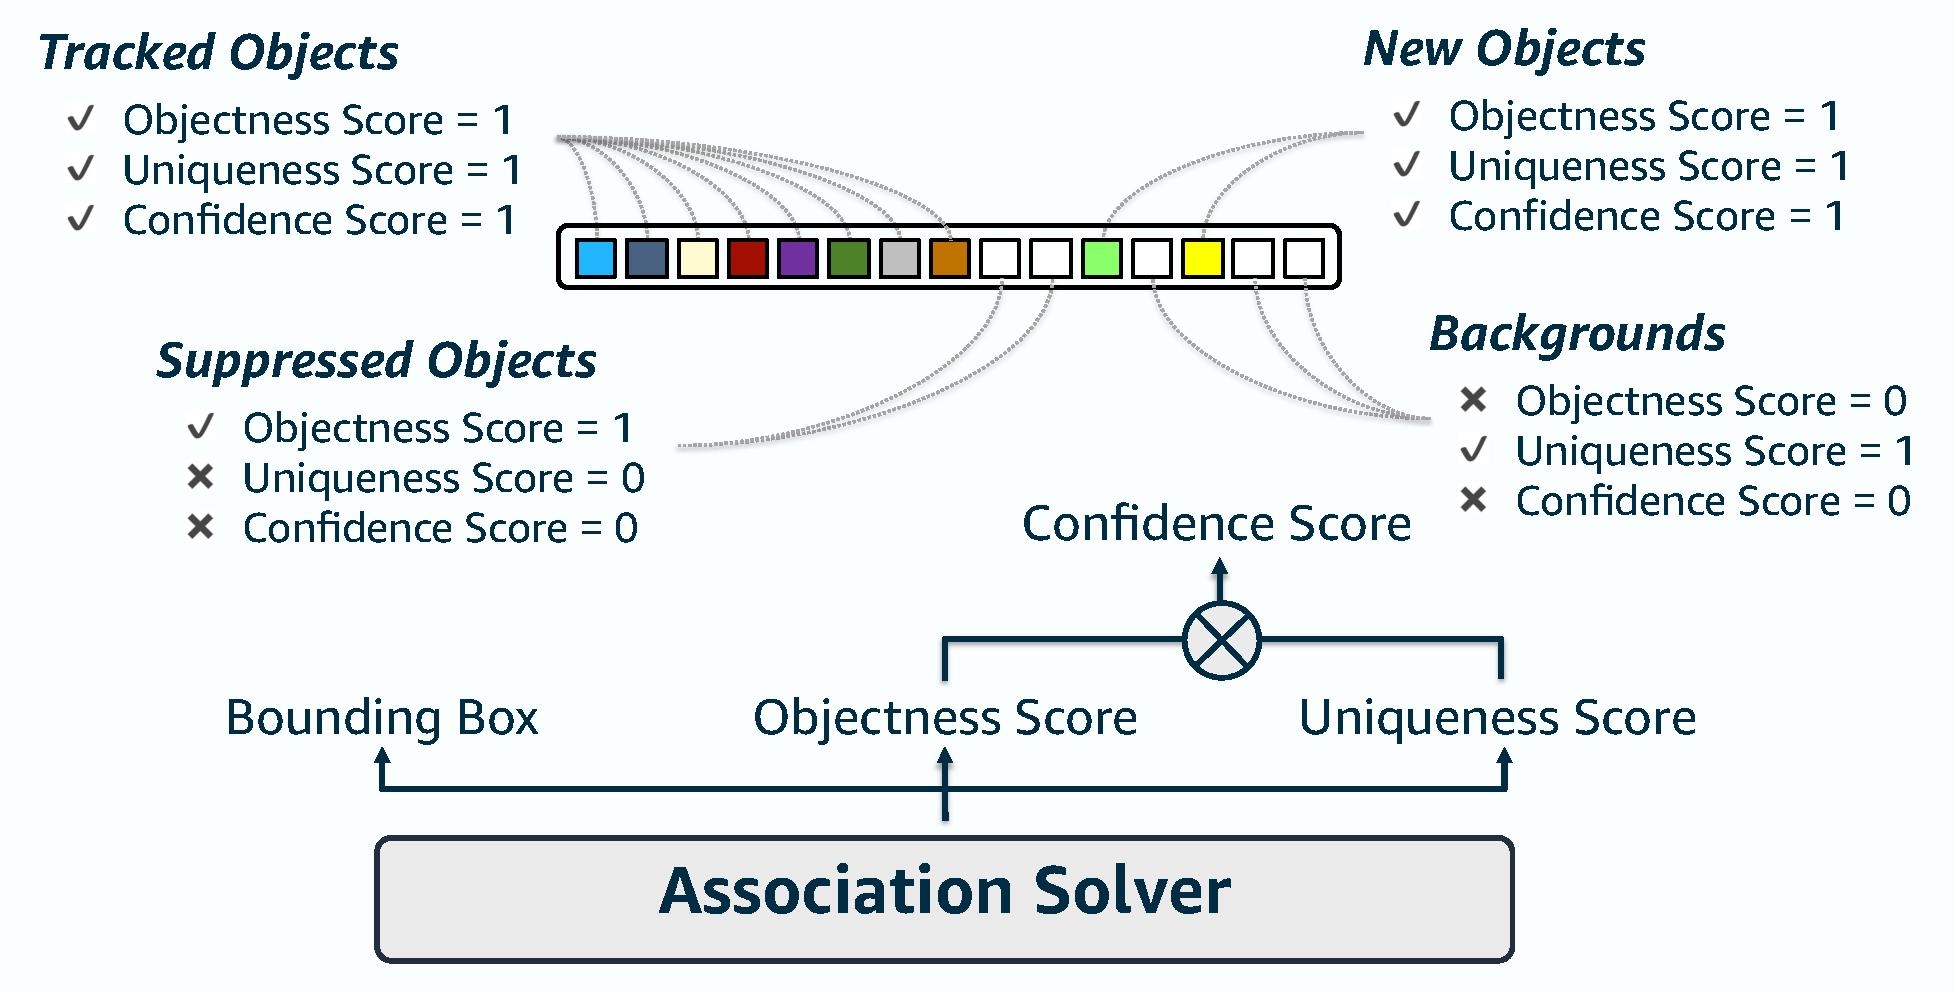
\includegraphics[width=0.5\textwidth]{figures/asso_module.pdf}
    \vspace{-6.0mm}
    \caption{\textbf{Illustration of ground truth assignment} to tracked objects, new objects, suppressed objects, and backgrounds. We show the assigned groundtruth scores for each type of entry.}
    \label{fig:asso_solver}
    \vspace{-4.0mm}
\end{figure}

\subsection{Training MeMOT}
\label{sec:method:training}

We supervise MeMOT with the \textit{tracking loss} computed on the $o_i^t$, $u_i^t$, $\mathbf{b}_i^t$ following the assignment process above as
%
\begin{equation}
%\small
    L_{tck} = \lambda_{cls}(L'_{obj}+L'_{uni})+\lambda_{L_1}L'_{bbox}+\lambda_{iou}L'_{iou},
\end{equation}
%
where $\lambda$s are hyper-parameters for weight scaling, $L_{obj}$ and $L_{uni}$ are focal loss on objectness scores and uniqueness scores, $L_{bbox}$ is L1 loss for bounding box regression, $L_{iou}$ is the generalized IoU loss~\cite{rezatofighi2019generalized}.

Additionally, we apply a detection loss to the proposal embedding similar to Deformable DETR's~\cite{zhu2020deformable} to enhance MeMOT's localization capability.
Specifically, we attach an auxiliary linear decoder to the proposal embedding to output bounding boxes and object classification scores. We then assign the object instances to them as in normal object detection tasks~\cite{zhu2020deformable} and similarly compute the loss as
%
\begin{equation}
%\small
   L_{det} = \lambda_{cls}L_{obj}+\lambda_{L_1}L_{bbox}+\lambda_{iou}L_{iou}.
\end{equation}
%
Note the auxiliary decoder is discarded after training. 

% , which is matched by the Hungarian algorithm, while those for the $\Theta_D$'s are determined by object identities (\ie, each query is responsible for a track).
% Formally, given the prediction results from the $\Theta_H$ decoder and $\Theta_D$ as $\hat{Y}_\tau$ and $\hat{Y'}_\tau$, respectively, their \textit{matched} ground truths are $Y_\tau$ and $Y'_\tau$ (depending on whether the object identity is considered), the losses are formulated as:
% %
% \begin{equation}
% \footnotesize
%     \begin{split}
%     L_{det}(Y_i,\hat{Y}_i) = &\lambda_{cls}L_{obj}+\lambda_{L_1}L_{bbox}+\lambda_{iou}L_{iou}, \\ 
%      L_{tck}(Y'_i,\hat{Y'}_i) = & \lambda_{cls}(L'_{obj}+L'_{uni})+\lambda_{L_1}L'_{bbox}+\lambda_{iou}L'_{iou},
%     \end{split}
% \end{equation}
% %
% where $\lambda$s are hyper-parameters for weight scaling, $L_{obj}$ and $L_{uni}$ are focal loss on objectness scores and uniqueness scores, $L_{bbox}$ is L1 loss for bounding box regression, $L_{iou}$ is the generalized IoU loss~\cite{rezatofighi2019generalized}.

%$L_{cls}$ is the objectness score $\hat{Y}_i$ and confidence score for $\hat{Y'}_i$ (defined in Eq.~\ref{eq:score}).

Following MOTR~\cite{zeng2021motr}, we compute the tracking loss in a clip by the sum of all individual track queries' losses normalized by the total number of object instances.
For a clip with $T$ frames, the overall loss $L_{clip}$ is a combination of the tracking loss and auxiliary detection loss as:
%
\begin{equation}
    \footnotesize
    \begin{split}
    L_{clip} &= \lambda_{tck}L_{clip-tck}+\lambda_{det}L_{clip-det} \\
    &=\frac{\lambda_{tck}}{\sum_{t=0}^{T} N_t}\sum_{t=0}^T\sum_{i=0}^{|\mathbi{Q}^t_{tc}, \mathbi{Q}^t_{pro}|}{L_{tck}^{(i, t)}}+\frac{\lambda_{det}}{T}\sum^T_{t=0}\frac{1}{N_t}\sum_{j=0}^{|\mathbi{Q}^t_{pro}|}L_{det}^{(j, t)},
    \end{split}
    \label{eq:cliploss}
\end{equation}
%
where $\lambda_{tck} \in \mathbb{R}$ and $\lambda_{det} \in \mathbb{R}$ are the loss weights for balancing the tracking loss and the auxiliary detection loss, respectively. 
Here $N_t$ denotes the total number of visible objects in the frame at time $t$.

%(\ie, new objects plus tracked objects) of bounding boxes in frame $t$.
In this section, we leverage the \snact\  to empirically validate the techniques introduced in \Cref{sec:techniques}. First, to concretize the capability gap between open-source and closed LLMs, we demonstrate that OpenAI GPT-4 API can have substantially higher success rate than representative open-source LLMs in~\Cref{subsec:cap_gap}. 
We then show in~\Cref{subsec:boost} that the simple techniques in~\Cref{sec:techniques} can boost open-source LLMs to achieve success rates competitive to in-context-learning with GPT-4 APIs\footnote{GPT-4 tuning APIs were not released by the time this work is done.} in four out of the eight tasks.
Through ablation studies in~\Cref{subsec:abl}, we additionally show that model alignment does the heavy lifting for boosting open-source LLMs, while system prompt and in-context learning robustify LLMs for further improvement. 

\subsection{Experiment Setup}
To establish strong baselines, we use GPT-4 API as the representative closed LLM in our study because it attains the leading accuracy in mainstream NLP tasks. 
In our study, we compare LLAMA-30B \cite{touvron2023llama}, StarCoder \cite{li2023starcoder} and CodeGen-16B-mono \cite{nijkamp2022codegen} to GPT-4. LLAMA represents open research models, while StarCoder and CodeGen are publicly available for both research and commercial purposes. We choose these three models due to their superior performance on \snact\  among open-source models as shown in~\Cref{tab:baselines_over_models}\footnote{Surprisingly, we observe that for tool manipulations, open-source LLMs instruction-tuned for conventional NLP tasks do not outperform their base models before tuning.}. 
In our experiments, we consider the zero-shot setting as the out-of-the-box configuration where only API documentation is provided without any demonstration examples. We use this configuration to understand the initial gap in capabilities among models. We then incorporate all available techniques on top of this initial configuration to assess their benefits. 
For the original Tabletop dataset~\cite{liang2022code}, which includes examples in a few-shot setting without explicit API definitions, we only evaluate settings with in-context demonstrations. 
More detailed setup information is included in \Cref{sec:app_exp_details}. We run each job 3 times with different random seeds and report average accuracy. The variation is minimal, so we ignore them in the main paper but report them in appendix.





\subsection{Capability Gap}
\label{subsec:cap_gap}
\Cref{tab:baselines} exhibits significant disparities in tool manipulation between the closed GPT-4 API and open-source models in the out-of-the-box zero-shot setting. 
For simpler tasks, namely Open Weather and the Cat API, which require only one API call for each goal, the open-source models exhibit success rates up to $74\%$ lower than GPT-4. 
Furthermore, on all the remaining tasks other than the Webshop, none of the LLAMA, the StarCoder and the CodeGen model can reach meaningful accuracy or compare with GPT-4. 
These results highlight an opportunity to enhance open-source LLMs.
% for tool manipulation.
% 1. Large gap across tasks
% 2. Some tasks demonstrate zero.
% 3. One interesting observation is that in context.

\begin{table}[]
\caption{Capability gap in tool manipulation is substantial between closed API and open-source LLMs in the out-of-the-box zero-shot setting. Using model alignment, the in-context demonstration retriever and the system prompt, open-soured LLMs attain significant boost in success rate. GPT-4 is enhanced with the retriever and system prompt.
% ; model alignment tuning does not apply to GPT-4 because tuning API is not available when we carry out the experiment.
Tabletop is only evaluated in the few-shot fashion. 
% Average success rate over 3 random seeds are reported. 
}
\label{tab:baselines}
\begin{adjustbox}{max width=\textwidth}

\setlength{\tabcolsep}{4pt}
\begin{tabular}{@{}cccccccccc@{}}
\toprule
                                          & \textbf{Open}                           & \textbf{The Cat}                    & \textbf{Home}        & \textbf{Trip}        & \textbf{Google}      &                                        & \multicolumn{2}{c}{\textbf{WebShop}}        &                                     \\
\multirow{-2}{*}{\textbf{Task}}           & {\color[HTML]{1F1F1F} \textbf{Weather}} & {\color[HTML]{1F1F1F} \textbf{API}} & \textbf{Search}      & \textbf{Booking}     & \textbf{Sheets}      & \multirow{-2}{*}{\textbf{VirtualHome}} & \textbf{Long}        & \textbf{Short}       & \multirow{-2}{*}{\textbf{Tabletop}} \\
\midrule
\textit{\textbf{Zero-shot Baseline}}      & \multicolumn{1}{l}{}                    & \multicolumn{1}{l}{}                & \multicolumn{1}{l}{} & \multicolumn{1}{l}{} & \multicolumn{1}{l}{} & \multicolumn{1}{l}{}                   & \multicolumn{1}{l}{} & \multicolumn{1}{l}{} & \multicolumn{1}{l}{}                \\
GPT-4                                          & 81.3            & 97.4            & 76.6            & 91.5            & 5.7             & 40.8 / 8.0  & \multicolumn{2}{c}{0.0}                    & -                    \\
LLaMA-30b                                     & 39.0            & 49.0            & 0.0             & 0.0            & 0.0             & 78.0 / 0.3  & \multicolumn{2}{c}{0.0}                    & -                    \\
StarCoder                                     & 32.0            & 71.0            & 7.0             & 13.3            & 5.9             & 22.0 / 3.7  & \multicolumn{2}{c}{0.0}                    & -                    \\
CodeGen-16B-mono                              & 7.0           & 78.0            & 0.0             & 0.0            & 1.4             & 4.0/ 1.0  & \multicolumn{2}{c}{0.0}                    & -                    \\

\midrule
\textit{\textbf{Enhanced w/ techniques}}      & \multicolumn{1}{l}{}                    & \multicolumn{1}{l}{}                & \multicolumn{1}{l}{} & \multicolumn{1}{l}{} & \multicolumn{1}{l}{} & \multicolumn{1}{l}{}                   & \multicolumn{1}{l}{} & \multicolumn{1}{l}{} & \multicolumn{1}{l}{}                \\
GPT-4                                      & 99.0                                    & 98.0                                & 98.0                 & 99.2                 & 68.6                 & 29.0 / 21.7                            & 0.0                  & 0.0                  & 83.8                                \\
LLaMA-30b                                     & 100.0           & 94.0            & 87.0            & 85.8            & 2.9             & 16.0 / 24.3 & 0.0             & 0.0             & 7.5             \\
StarCoder                                     & 99.0            & 97.0            & 83.0            & 80.8            & 21.2            & 31.0 / 18.4 & 0.0             & 0.0             & 13.9            \\
CodeGen-16B-mono                              & 97.7            & 99.0            & 82.0            & 77.5            & 19.8            & 29.0 / 17.2 & 0.0             & 3.5             & 16.2                    \\
\bottomrule
\end{tabular}
\end{adjustbox}
% \vspace{-1em}
\end{table}


% \begin{table}[]
% \caption{Capability gap in tool manipulation is substantial between closed API and open-source LLMs in the out-of-the-box zero-shot setting. Using model alignment, the in-context demonstration retriever and the system prompt, open-soured LLMs attain significant boost in success rate. GPT-4 is enhanced with the retriever and system prompt.
% % ; model alignment tuning does not apply to GPT-4 because tuning API is not available when we carry out the experiment.
% Tabletop is only evaluated in the few-shot fashion.
% }
% \label{tab:baselines}
% \begin{adjustbox}{max width=\textwidth}

% \setlength{\tabcolsep}{4pt}
% \begin{tabular}{@{}cccccccccc@{}}
% \toprule
%                                           & \textbf{Open}                           & \textbf{The Cat}                    & \textbf{Home}        & \textbf{Trip}        & \textbf{Google}      &                                        & \multicolumn{2}{c}{\textbf{WebShop}}        &                                     \\
% \multirow{-2}{*}{\textbf{Task}}           & {\color[HTML]{1F1F1F} \textbf{Weather}} & {\color[HTML]{1F1F1F} \textbf{API}} & \textbf{Search}      & \textbf{Booking}     & \textbf{Sheets}      & \multirow{-2}{*}{\textbf{VirtualHome}} & \textbf{Long}        & \textbf{Short}       & \multirow{-2}{*}{\textbf{Tabletop}} \\
% \midrule
% \textit{\textbf{Zero-shot Baseline}}      & \multicolumn{1}{l}{}                    & \multicolumn{1}{l}{}                & \multicolumn{1}{l}{} & \multicolumn{1}{l}{} & \multicolumn{1}{l}{} & \multicolumn{1}{l}{}                   & \multicolumn{1}{l}{} & \multicolumn{1}{l}{} & \multicolumn{1}{l}{}                \\
% GPT-4                                      & 70.0                                    & 80.0                                & 70.0                 & 45.0                 & 5.7                  & 29.0 / 9.5                             & \multicolumn{2}{c}{0.0}                     & -                                   \\
% LLaMA-30b                                 & 6.0                                     & 5.0                                 & 0.0                  & 0.0                  & 0.0                  & 3.0 / 0.1                              & \multicolumn{2}{c}{0.0}                     & -                                   \\
% LLaMA-30b                                 & 6.0                                     & 5.0                                 & 0.0                  & 0.0                  & 0.0                  & 3.0 / 0.1                              & \multicolumn{2}{c}{0.0}                     & -                                   \\
% CodeGen-16B-mono                          & 12.0                                    & 47.0                                & 0.0                  & 0.0                  & 0.0                  & 0.0 / 0.6                              & \multicolumn{2}{c}{0.0}                    & -                                   \\
% \midrule
% \textit{\textbf{Enhanced w/ techniques}}      & \multicolumn{1}{l}{}                    & \multicolumn{1}{l}{}                & \multicolumn{1}{l}{} & \multicolumn{1}{l}{} & \multicolumn{1}{l}{} & \multicolumn{1}{l}{}                   & \multicolumn{1}{l}{} & \multicolumn{1}{l}{} & \multicolumn{1}{l}{}                \\
% GPT-4                                      & 99.0                                    & 98.0                                & 98.0                 & 99.2                 & 68.6                 & 29.0 / 21.7                            & 0.0                  & 0.0                  & 83.8                                \\
% GPT-4                                      & 99.0                                    & 98.0                                & 98.0                 & 99.2                 & 68.6                 & 29.0 / 21.7                            & 0.0                  & 0.0                  & 83.8                                \\
% LLaMA-30b & 100.0 & 95.0 & 86.0 & 85.8 & 2.9 & 15.0 / 26.4 & 0.0 & 0.0 & 7.6 \\
% CodeGen-16B-mono                          & 99.0                                    & 99.0                                & 83.0                 & 76.7                 & 18.6                 & 37.0 / 19.3                            & 0.0                  & 13.2                 & 16.2                               \\
% \bottomrule
% \end{tabular}
% \end{adjustbox}
% % \vspace{-1em}
% \end{table}
\subsection{Boosting open-source LLMs}
\label{subsec:boost}
To boost the open-source LLMs, we first perform model alignment using programmatially generated data. We then apply a system prompt and a 3-shot demonstration retriever during inference. Given GPT-4 does not provide tuning APIs, we enhance the out-of-the-box GPT-4 with the same system prompt and demonstration retriever as the baseline. The improvements from the combined enhancement techniques are shown in~\Cref{tab:baselines}, where the success rates of the open-source LLMs can improve up to $90\%$. As a result, the open-source models achieve competitive or better success rates on 4 out of 8 tasks, including Open Weather, the Cat API, VirturalHome and WebShop. Moreover, on Home Search and Trip Booking, the gap between the LLAMA model and the GPT-4 API is reduced to $11\%$ and $13.4\%$ respectively, compared to the initial gap of up to $91\%$. Despite the fact that open-source models are still lagging behind on the Google Sheets and Tabletop, these observations show that \emph{our recipe can significantly improve the performance of open-source LLMs and attain success rates comparable to GPT-4 API on many of the \snact\  tasks}.

\paragraph{Human supervision} To identify the practicality of an enhancement recipe, the amount of required human supervision is a crucial factor. In our approach, human supervision is primarily in the form of in-context demonstration examples and alignment data templates.
Regarding the demonstration examples, we provide $10$ to $83$ examples for each task as shown in~\Cref{tab:all_tasks}, except for WebShop given its difficulty in advanced reasoning.
% and the ones in VirtualHome, Webshop and Tabletop are already provided in their original datasets.
As shown in~\Cref{tab:training_data}, the number of templates for alignment data is typically less than $100$ for each task. We observe that providing these supervisions takes one developer day on average, making it practical in terms of the time cost on human supervision.
% \comment{QT: need the statistics on volume of templates for each task and maybe also total generated alignment example count}


\paragraph{Remaining challenges} In our experiments, we observe that the boosted open-source LLMs still have relatively low success rates on tasks that require advanced reasoning, such as Google Sheets, WebShop and Tabletop tasks. This implies the need to further enhance the reasoning capabilities of open-source models. We are excited about the prospect of more exploration from the community to address the challenges for tool manipulation on these complex tasks.



% % 1. Compared 3 trick open sourced to GPT + 2 things for GPT
% 2. Discuss a few examples
% 3. Supervision needed
% 4. Remaining challenges

\subsection{Ablation Study}
\label{subsec:abl}

\begin{wraptable}[14]{r}{6cm}
\vspace{-12pt}
\caption{The number of \snact~tasks improved (+N) or hurt (-N) over the baselines when adding or dropping techniques.}
\label{tab:breakdown}
\begin{adjustbox}{max width=\linewidth}
\setlength{\tabcolsep}{2pt}
\begin{tabular}{@{}lccc@{}}
\toprule
               & LLaMA & StarCoder & CodeGen \\
\midrule
\textbf{Zero-shot} & - & - & -                                                \\
+ Sys. Prompt       & +4 & +4 & +4                                               \\
+ 3-shot & +8 & +8 & +8                                                \\
+ Alignment   & +7 & +7 &+7                                     \\  
\midrule
\textbf{Full system} & - & - & -                                                \\
- Sys. Prompt       & -0 & -2 & -3                                                \\
- 3-shot    & -3 & -4 & -5                                                 \\
- Alignment  & -5 & -5 & -7                                      \\        
\bottomrule
\end{tabular}
\end{adjustbox}
\end{wraptable} 
% To break down the contribution of model alignment, in-context demonstration and sysmtem prompts, we ablate these techniques in two ways in~\Cref{tab:breakdown}. We first apply one technique a time on top of the out-of-the-box zero-shot configuration and show the impacts in isolation. We then take the combination of the techniques and remove one at a time to evaluate the relative contributions in the context of the full system.
% The full results of the experiments in this section can be found in \Cref{tab:baselines_over_techniques}.

% \paragraph{Impact of techniques} 
% As seen in~\Cref{tab:breakdown}, both 3-shot in-context demonstration and model alignment can bump up the success rate of all the tasks, while system prompts only boosts simple tasks requiring relatively fewer number of API call for each goal.

% \paragraph{System ablation} In the context of full system with all three techniques, we can observe that solely removing model alignment triggers success rate degradation in up to 7 tasks in~\Cref{tab:breakdown}, while removing either in-context demonstration or system prompt hurts up to 5 tasks. We notice that the tasks that are not significantly hurt when removing techniques are the ones that have relatively low success rate (usually <20\%) even in the full system. Thus those accuracy changes are subject to high variance and fluctuation.


% To break down the contribution of model alignment, in-context demonstration and sysmtem prompts, we ablate these techniques in two ways. 
We break down the contribution of the techniques in two ways.
First, we apply each technique individually on top of the out-of-the-box zero-shot configuration and evaluate its impact. 
As shown in~\Cref{tab:breakdown}, both the 3-shot in-context demonstration and model alignment techniques bump up the success rates across all tasks, while the system prompt only benefits simple tasks that involve relatively fewer API calls for each goal.

Next, we consider the combination of all techniques and remove them one at a time to evaluate their relative contributions within the full system. As shown in in~\Cref{tab:breakdown}, solely removing model alignment triggers success rate degradation in up to 7 tasks, while removing either in-context demonstration up to 5 tasks and dropping system prompt up to 3. We notice that the tasks that are not significantly impacted when removing techniques are typically the ones with relatively low success rate (usually <20\% even in the full system). Thus, those accuracy changes are hypothetically subject to high variance and fluctuation.
The full results from the experiments in this section can be found in \Cref{tab:baselines_over_techniques}.



% \textbf{Greatly reduce the gap between open- and close-source models}. There is a great gap between open-source models and closed models out-of-the-box in the zero-shot setting. However, when armed with the techniques we provided, the open-source model are dramatically improved from almost non-usable (e.g. the accuracy of LLaMA is below 10\% for most of the tasks) to GPT-4 level on 6 out of 8 tasks, even though the GPT-4 can also benefit from those techniques. 

% \textbf{Our proposed techniques are effective}. Comparing with the zero-shot baseline, every single technique - system prompting, few-shot learning, alignment tuning - can individually bump up the model performance universally across different tasks. Alignment tuning and in-context learning can each close the gap in 5 out of 8 tasks, while deliminate major gap in the rest, when comparing with the GPT-4 zero-shot baseline.

% \textbf{Minimum human supervision's needed.} Show the amount of human labor needed for curate demonstration examples and tuning templates. 

% \subsection{Techniques Contribution Breakdown}
% \label{subsec:abl}


% To understand the contribution of each task, we compute the average success rate of the first 4 tasks on LLaMA and CodeGen, by incrementally removing techniques from the joint setting. We exclude the last four tasks from \snact~ because of their highly variant results (we didn't fully exploit the tuning) \comment{rephrase me to align with 6.1}. As shown in \Cref{tab:breakdown}, combining the three techniques together delivers the best model performance, indicating the techniques are complimentary to each other. Also, we confirm again that tuning is the most beneficial techniques to bump up the open-source model accuracy.

% Describe limitations and any potential negative societal impacts


In this paper, we answer the question \emph{can we enhance open-source LLMs to compete with leading closed LLM APIs in tool manipulation, with practical amount of human supervision}. 
Drawing from our observations of the common tool manipulation failures and insights from the literature on conventional NLP tasks with LLM, we propose to instantiate model alignment with programmatical data generation, system prompts, and in-context demonstration retrievers to improve the tool manipulation capability of open-source models.
To comprehensively evaluate the impact of these techniques, we create the \textit{\snact}, a benchmark consisting of diverse software tools for real-world tasks. 
Our results demonstrate that these techniques can make the leading open-source LLMs competitive with the OpenAI GPT-4 in $4$ out of $8$ \snact\  tasks, all achieved with a practical amount of human labeling effort.

\section{Additional Results}
\subsection{GPT-3 Experiments} 
\label{sec:gpt3}
\begin{table}[ht]
    \centering
\begin{tabular}{c | cc}
\toprule
 & PaLM-540B & GPT-3 \\ \midrule
HotpotQA (exact match) & 29.4 & \textbf{30.8} \\
ALFWorld (success rate \%) & 70.9 & \textbf{78.4} \\ 
\bottomrule
\end{tabular}%
    \caption{\model{} prompting results using PaLM-540B vs.\,GPT-3 (text-davinci-002, greedy decoding). On HotpotQA, we randomly sample a subset of 500 validation questions. On ALFWorld, we use all 134 unseen validation task instances, and use the best prompt set according to PaLM-540B.}
    \label{tab:gpt3}
\end{table}
We run additional GPT-3~\citep{brown2020language} experiments to confirm \model{} prompting performance is general across different large language models. As shown in Table~\ref{tab:gpt3}, GPT-3 (text-davinci-002, greedy decoding) consistently outperforms PaLM-540B on HotpotQA and ALFWorld, possibly because it is finetuned with human instruction following. This indicates ReAct prompting is effective across different large language models on different tasks.
The code for these experiments are at \url{https://react-lm.github.io/}.
\subsection{\model{} obtains up-to-date knowledge on HotpotQA}
\begin{figure}[ht]
    \centering
    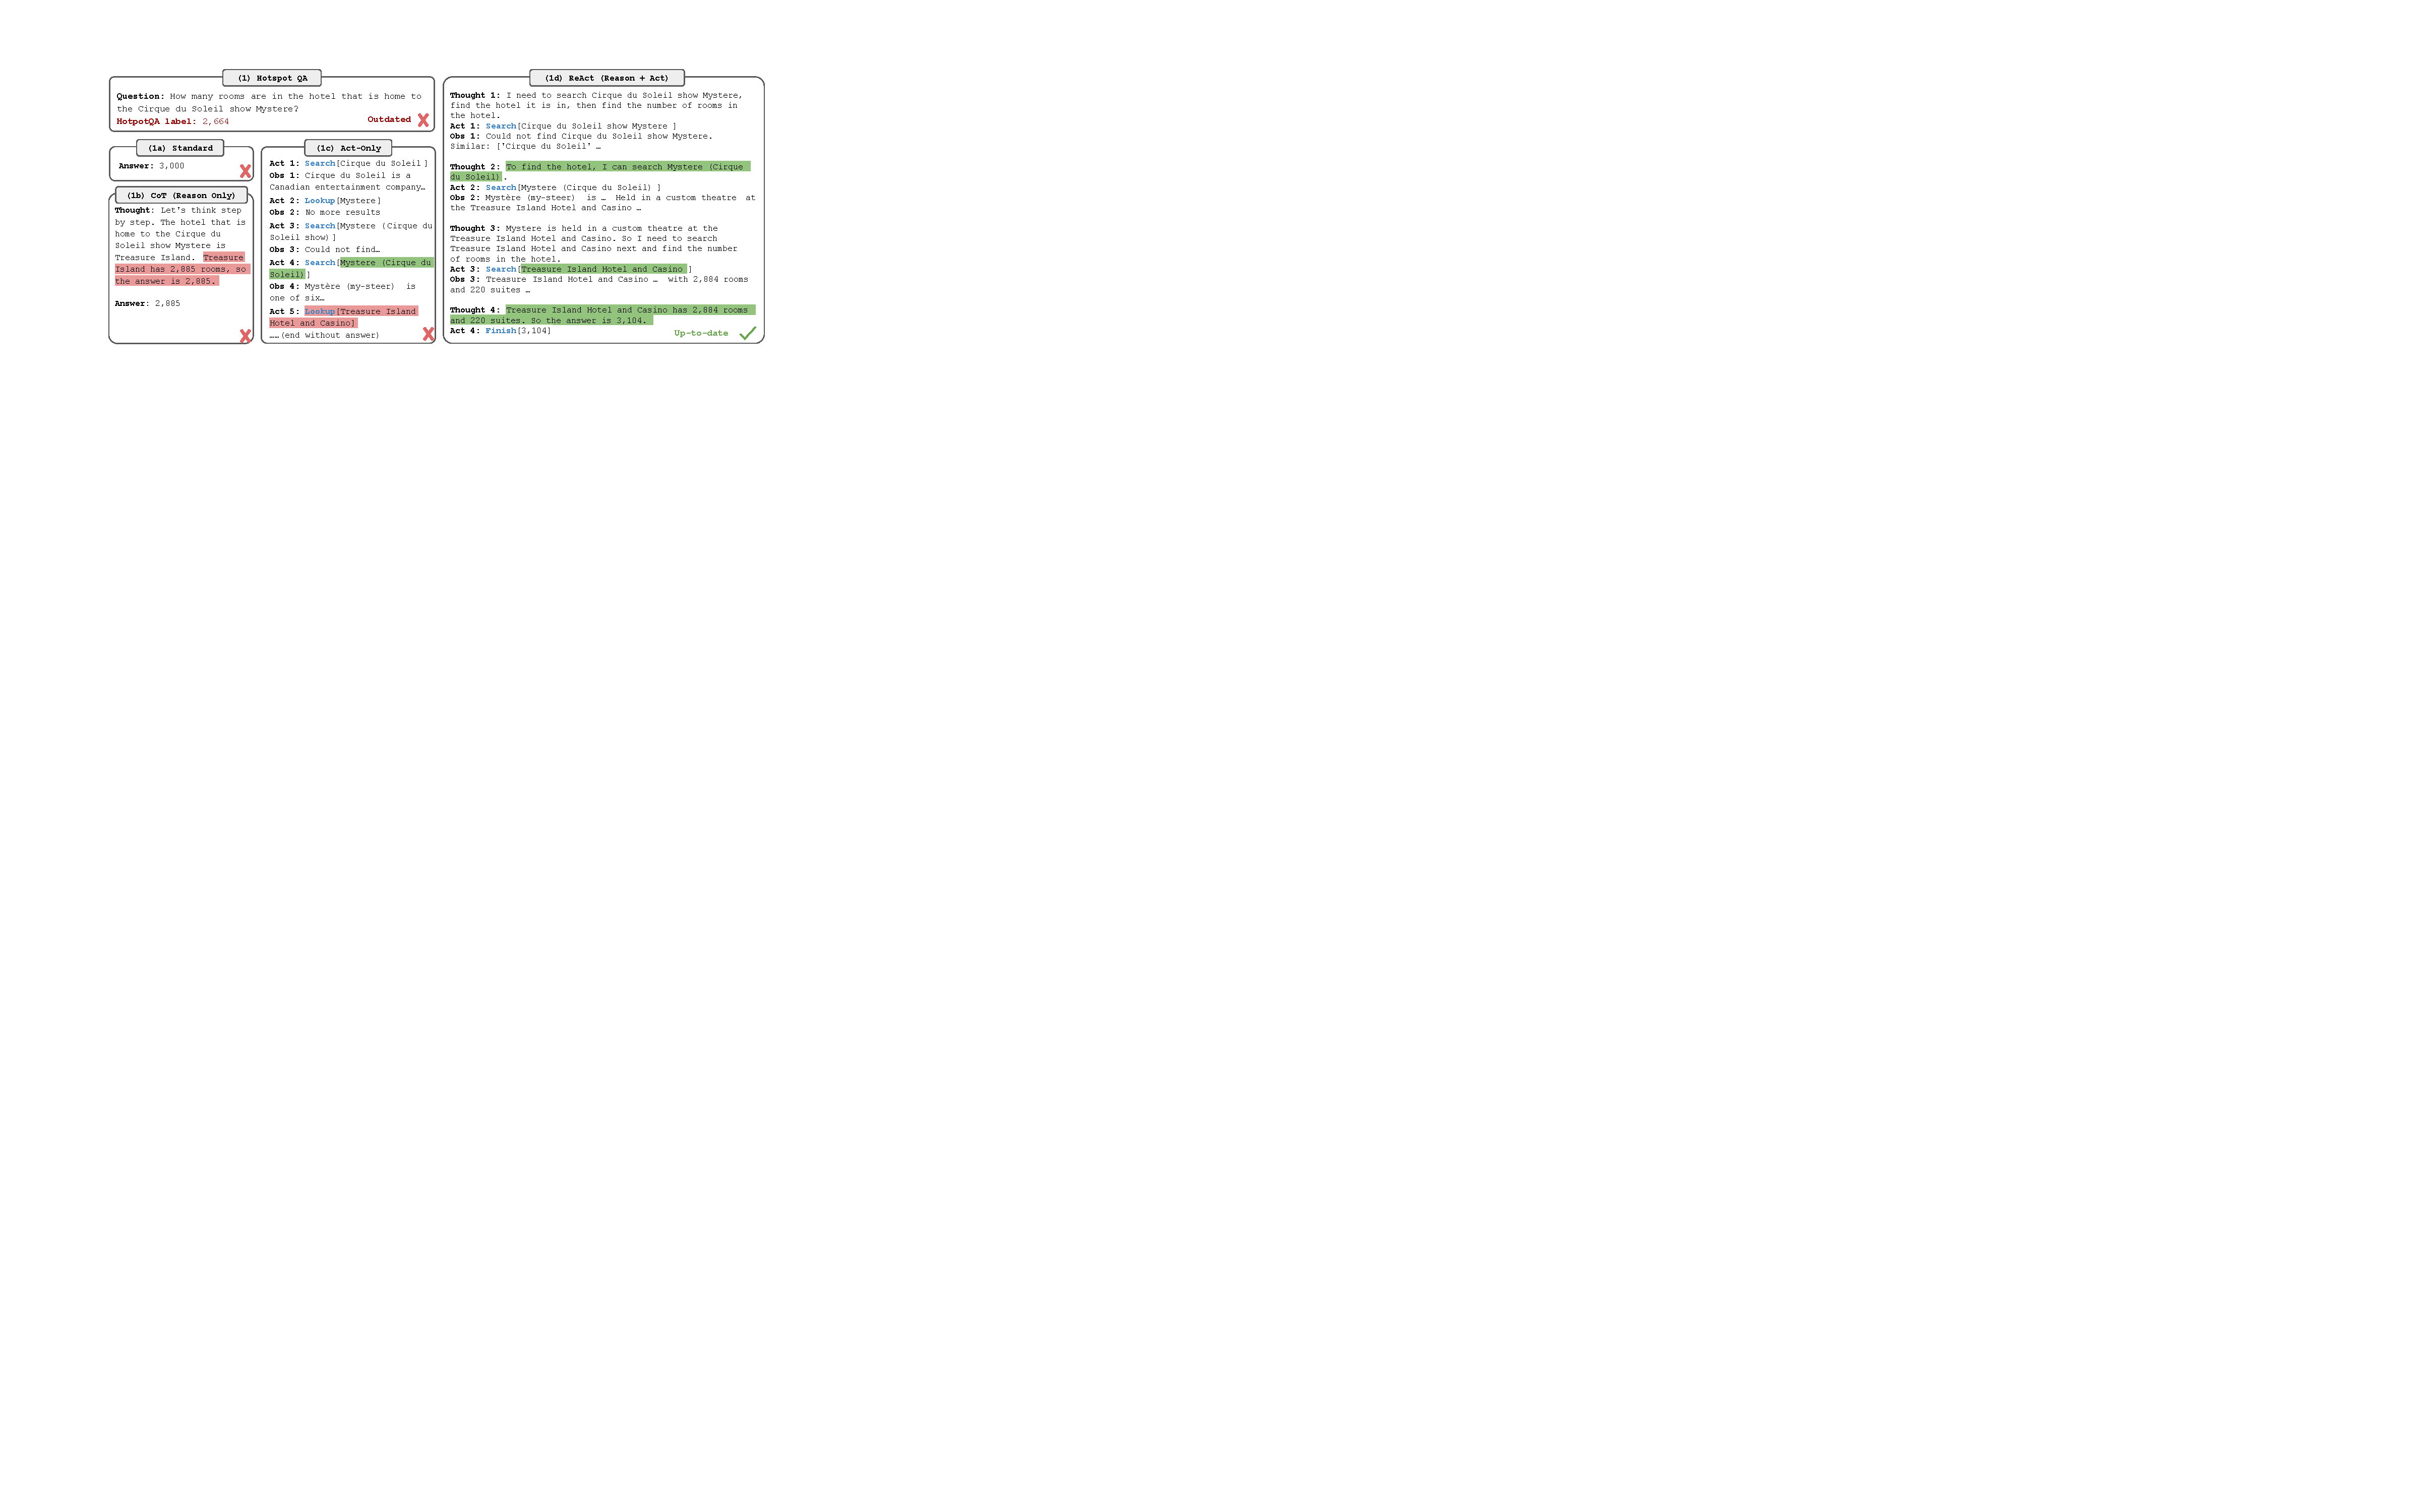
\includegraphics[width=\textwidth]{iclr2023/figure/date.pdf}
    \caption{
    {
    Another example HotpotQA question, where the original label is outdated. Only \model{} is able to obtain the up-to-date answer thanks to real-world web interaction plus reasoning.}
    }
    \label{fig:date}
    \vspace{-10pt}
\end{figure}

During trajectory inspection, we also find that sometimes \model{} does not agree with dataset labels as the labels themselves could be outdated. For example, as shown in Figure~\ref{fig:date}, the question asks about the size of a hotel, which increased from the HotpotQA construction time. While \palm{} and \reason{} give wrong answers due to hallucination, \act{} fails despite the access of real-world web interaction, due to a lack of reasoning to guide how to interact with the Internet for QA. Only \model{} is able to retrieve up-to-date information from the Internet and provide a reasonable answer. Therefore, better incorporation of reasoning abilities might benefit recent Internet-augmented language models~\citep{nakano2021webgpt,lazaridou2022internet,shuster2022language} for up-to-date task solving. 
\subsection{Human-in-the-loop behavior correction on AlfWorld} 
\begin{figure}[ht]
    \centering
    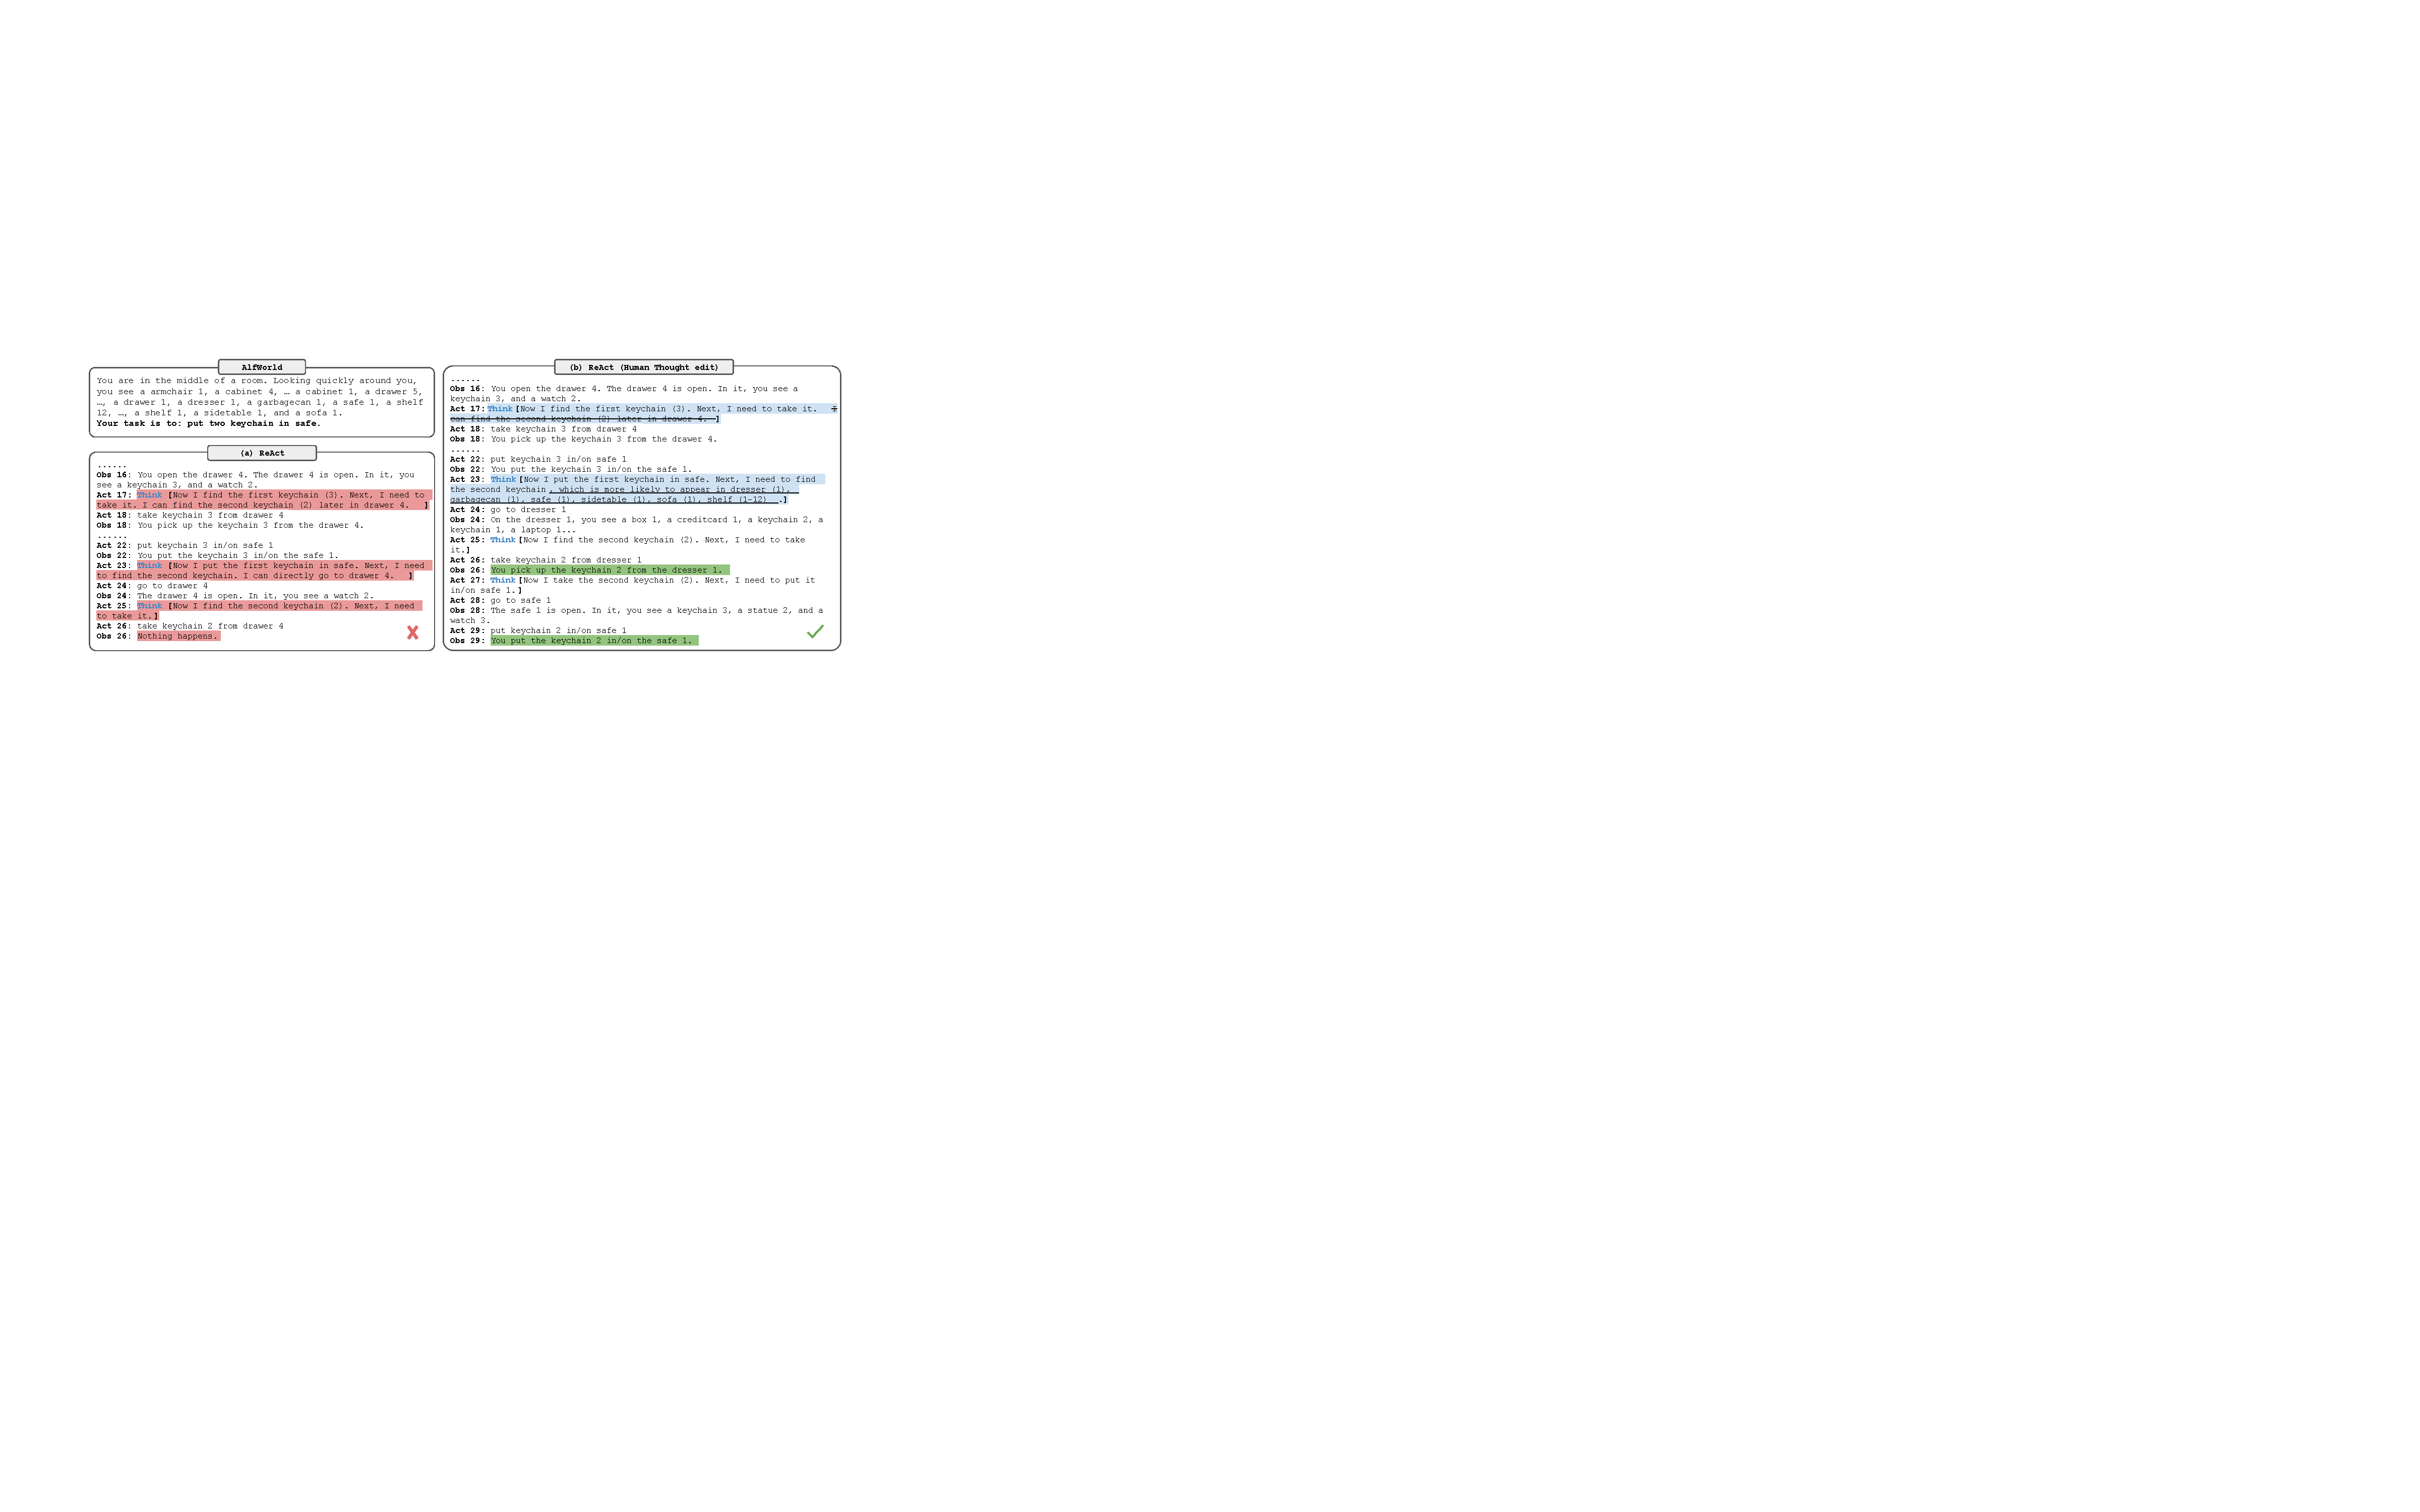
\includegraphics[width=\textwidth]{iclr2023/figure/human_edit.pdf}
    \caption{
    A human-in-the-loop behavior correction example with \model{} in AlfWorld. 
    (a) \model{} trajectory fails due to a hallucinating thought (Act 17).
    (b) By a human simply editing two thoughts (Act 17, 23), the \model{} trajectory produces desirable reasoning traces and actions and succeeds.
    }
    \label{fig:edit}
    \vspace{-10pt}
\end{figure}

We also explore human-in-the-loop interaction with \model{}, to allow a human to inspect and edit \model's reasoning traces. Figure~\ref{fig:edit} shows that
by simply removing a hallucinating sentence in Act 17 and adding some hints in Act 23, \model{} can be made to change its behavior drastically to align with these human thought edits and succeed in the task. 
From a human perspective, solving such a task becomes significantly easier, from typing tens of actions to only editing a couple of thoughts, which enables new forms of human-machine collaboration.
We note that such a policy edit on-the-go is difficult for \act{} and previous RL methods, as a human cannot change the model parameters, and changing a few actions might not edit the rest of the model behavior. 
This paradigm is also more than human dialogue to update the goal or subgoal as in \citet{huang2022inner} --- while editing \model{} thoughts can do these, it can also modify the model's internal belief, reasoning styles, or anything the flexible thought space supports, for better task solving. 
We believe this is an exciting direction for human alignment and leave more systematic study as future work.

\section{Experiment Details}
\subsection{HotpotQA Finetuning Details}
\label{sec:hotpot_finetune}
For all finetuning we use a batch size of 64.
On PaLM-8B, we finetune \model{} and \act{} methods for $4,000$ steps and \palm{} and \reason{} methods for $2,000$ steps. 
On PaLM-62B, we finetune \model{} and \act{} methods for $4,000$ steps and \palm{} and \reason{} methods for $1,000$ steps. 
We find \model{} and \act{} methods generally benefit from more training steps (and more training data), while  \palm{} and \reason{} methods degrade soon after finetuning.

\subsection{AlfWorld IM-Style Details}
\label{sec:alfworld_im}
For the IM-style ablation, the same expert trajectories used in \model{} are reannotated with dense external feedback thoughts within these trajectories, that limit \modelim{} to only think about (1) decomposing the current goal and (2) the current subgoal that needs to be completed. In particular, \modelim{} lacks thoughts that (1) determine when a subgoal is completed (2) determine what the next subgoal should be (3) inducing the LLM to refer to its internal pretraining knowledge to identify where items can be within the environment. 


\section{Prompts}
\label{sec:prompts}
\subsection{HotpotQA}
\begin{table}[H]
\scriptsize
\begin{minipage}{0.9\linewidth}
Hotpot QA Prompts
\centering
\ttfamily
\begin{tabular}{l p{0.9\linewidth}}
\midrule
\sethlcolor{cyan}\hl{Original} & \\
Question &  What is the elevation range for the area that the eastern sector of the Colorado orogeny extends into? \\
Answer &  1,800 to 7,000 ft\\
\\
Question &  Musician and satirist Allie Goertz wrote a song about the "The Simpsons" character Milhouse, who Matt Groening named after who?\\
Answer &  Richard Nixon\\
\\
Question &  Which documentary is about Finnish rock groups, Adam Clayton Powell or The Saimaa Gesture?\\
Answer &  The Saimaa Gesture\\
\\
Question &  What profession does Nicholas Ray and Elia Kazan have in common?\\
Answer &  director, screenwriter, actor\\
\\
Question &  Which magazine was started first Arthur's Magazine or First for Women?\\
Answer &  Arthur's Magazine\\
\\
Question &  Were Pavel Urysohn and Leonid Levin known for the same type of work?\\
Answer &  Yes\\


\midrule
\sethlcolor{red}\hl{\act} & \\
Question &  What is the elevation range for the area that the eastern sector of the Colorado orogeny extends into?\\
Action 1 &  Search[Colorado orogeny]\\
Observation 1 &  The Colorado orogeny was an episode of mountain building (an orogeny) in Colorado and surrounding areas.\\
Action 2 &  Lookup[eastern sector]\\
Observation 2 &  (Result 1 / 1) The eastern sector extends into the High Plains and is called the Central Plains orogeny.\\
Action 3 &  Search[High Plains]\\
Observation 3 &  High Plains refers to one of two distinct land regions: \\
Action 4 &  Search[High Plains (United States)]\\
Observation 4 &  The High Plains are a subregion of the Great Plains. From east to west, the High Plains rise in elevation from around 1,800 to 7,000 ft (550 to 2,130 m).[3]\\
Action 5 &  Finish[1,800 to 7,000 ft]\\
\\
Question &  Musician and satirist Allie Goertz wrote a song about the "The Simpsons" character Milhouse, who Matt Groening named after who?\\
Action 1 &  Search[Milhouse]\\
Observation 1 &  Milhouse Mussolini Van Houten is a recurring character in the Fox animated television series The Simpsons voiced by Pamela Hayden and created by Matt Groening.\\
Action 2 &  Lookup[named after]\\
Observation 2 &  (Result 1 / 1) Milhouse was named after U.S. president Richard Nixon, whose middle name was Milhous. \\
Action 3 &  Finish[Richard Nixon]\\
\\
Question &  Which documentary is about Finnish rock groups, Adam Clayton Powell or The Saimaa Gesture?\\
Action 1 &  Search[Adam Clayton Powell]\\
Observation 1 &  Could not find [Adam Clayton Powell]. Similar:  ['Adam Clayton Powell III', 'Seventh Avenue (Manhattan)', 'Adam Clayton Powell Jr. State Office Building', 'Isabel Washington Powell', 'Adam Powell', 'Adam Clayton Powell (film)', 'Giancarlo Esposito'].\\
Action 2 &  Search[Adam Clayton Powell (film)]\\
Observation 2 &  Adam Clayton Powell is a 1989 American documentary film directed by Richard Kilberg. The film is about the rise and fall of influential African-American politician Adam Clayton Powell Jr.[3][4] It was later aired as part of the PBS series The American Experience.\\
Action 3 &  Finish[The Saimaa Gesture]\\
\\
Question &  What profession does Nicholas Ray and Elia Kazan have in common?\\
Action 1 &  Search[Nicholas Ray]\\
Observation 1 &  Nicholas Ray (born Raymond Nicholas Kienzle Jr., August 7, 1911 – June 16, 1979) was an American film director, screenwriter, and actor best known for the 1955 film Rebel Without a Cause.\\
Action 2 &  Search[Elia Kazan]\\
Observation 2 &  Elia Kazan was an American film and theatre director, producer, screenwriter and actor.\\


\midrule \multicolumn{2}{r}{\textit{Continued on next page}} \\
\end{tabular}
\end{minipage}%
\end{table}


\begin{table}[H]
\scriptsize
\begin{minipage}{0.9\linewidth}
Hotpot QA Prompts -- Continued from previous page
\centering
\ttfamily
\begin{tabular}{l p{0.9\linewidth}}
\midrule
\\
Action 3 &  Finish[director, screenwriter, actor]\\
Question &  Which magazine was started first Arthur's Magazine or First for Women?\\
Action 1 &  Search[Arthur's Magazine]\\
Observation 1 &  Arthur's Magazine (1844--1846) was an American literary periodical published in Philadelphia in the 19th century. \\
Action 2 &  Search[First for Women]\\
Observation 2 &  First for Women is a woman's magazine published by Bauer Media Group in the USA.[1] The magazine was started in 1989. \\
Action 3 &  Finish[Arthur's Magazine]\\
\\
Question &  Were Pavel Urysohn and Leonid Levin known for the same type of work?\\
Action 1 &  Search[Pavel Urysohn]\\
Observation 1 &  Pavel Samuilovich Urysohn (February 3, 1898 - August 17, 1924) was a Soviet mathematician who is best known for his contributions in dimension theory.\\
Action 2 &  Search[Leonid Levin]\\
Observation 2 &  Leonid Anatolievich Levin is a Soviet-American mathematician and computer scientist. \\
Action 3 &  Finish[yes]\\
\midrule
\sethlcolor{green}\hl{\reason} & \\
Question &  What is the elevation range for the area that the eastern sector of the Colorado orogeny extends into?\\
Thought &  Let's think step by step. The eastern sector of Colorado orogeny extends into the High Plains. High Plains rise in elevation from around 1,800 to 7,000 ft, so the answer is 1,800 to 7,000 ft.\\
Answer &  1,800 to 7,000 ft\\
\\
Question &  Musician and satirist Allie Goertz wrote a song about the "The Simpsons" character Milhouse, who Matt Groening named after who?\\
Thought &  Let's think step by step. Milhouse was named after U.S. president Richard Nixon, so the answer is Richard Nixon.\\
Answer &  Richard Nixon\\
\\
Question &  Which documentary is about Finnish rock groups, Adam Clayton Powell or The Saimaa Gesture?\\
Thought &  Let's think step by step. Adam Clayton Powell (film) is a documentary about an African-American politician, not Finnish rock groups. So the documentary about Finnish rock groups must instead be The Saimaa Gesture.\\
Answer &  The Saimaa Gesture\\
\\
Question &  What profession does Nicholas Ray and Elia Kazan have in common?\\
Thought &  Let's think step by step. Professions of Nicholas Ray are director, screenwriter, and actor. Professions of Elia Kazan are director, producer, screenwriter, and actor. So profession Nicholas Ray and Elia Kazan have in common is director, screenwriter, and actor.\\
Answer &  director, screenwriter, actor\\
\\
Question &  Which magazine was started first Arthur's Magazine or First for Women?\\
Thought &  Let's think step by step. Arthur's Magazine was started in 1844. First for Women was started in 1989. 1844 (Arthur's Magazine) < 1989 (First for Women), so Arthur's Magazine was started first.\\
Answer &  Arthur's Magazine\\
\\
Question &  Were Pavel Urysohn and Leonid Levin known for the same type of work?\\
Thought &  Let's think step by step. Pavel Urysohn is a mathematician. Leonid Levin is a mathematician and computer scientist. So Pavel Urysohn and Leonid Levin have the same type of work.\\
Answer &  Yes\\


\midrule
\sethlcolor{yellow}\hl{\model} & \\
Question &  What is the elevation range for the area that the eastern sector of the Colorado orogeny extends into?\\
Thought 1 &  I need to search Colorado orogeny, find the area that the eastern sector of the Colorado orogeny extends into, then find the elevation range of the area.\\
Action 1 &  Search[Colorado orogeny]\\
Observation 1 &  The Colorado orogeny was an episode of mountain building (an orogeny) in Colorado and surrounding areas.\\
Thought 2 &  It does not mention the eastern sector. So I need to look up eastern sector.\\
Action 2 &  Lookup[eastern sector]\\
Observation 2 &  (Result 1 / 1) The eastern sector extends into the High Plains and is called the Central Plains orogeny.\\
Thought 3 &  The eastern sector of Colorado orogeny extends into the High Plains. So I need to search High Plains and find its elevation range.\\
Action 3 &  Search[High Plains]\\
Observation 3 &  High Plains refers to one of two distinct land regions  \\
Thought 4 &  I need to instead search High Plains (United States).\\
Action 4 &  Search[High Plains (United States)]\\

\midrule \multicolumn{2}{r}{\textit{Continued on next page}} \\

\end{tabular}
\end{minipage}%
\end{table}


\begin{table}[H]
\scriptsize
\begin{minipage}{0.9\linewidth}
Hotpot QA Prompts -- Continued from previous page
\centering
\ttfamily
\begin{tabular}{l p{0.9\linewidth}}
\midrule
\\
Observation 4 &  The High Plains are a subregion of the Great Plains. From east to west, the High Plains rise in elevation from around 1,800 to 7,000 ft (550 to 2,130 m).[3]\\
Thought 5 &  High Plains rise in elevation from around 1,800 to 7,000 ft, so the answer is 1,800 to 7,000 ft.\\
Action 5 &  Finish[1,800 to 7,000 ft]\\
\\
Question &  Musician and satirist Allie Goertz wrote a song about the "The Simpsons" character Milhouse, who Matt Groening named after who?\\
Thought 1 &  The question simplifies to "The Simpsons" character Milhouse is named after who. I only need to search Milhouse and find who it is named after.\\
Action 1 &  Search[Milhouse]\\
Observation 1 &  Milhouse Mussolini Van Houten is a recurring character in the Fox animated television series The Simpsons voiced by Pamela Hayden and created by Matt Groening.\\
Thought 2 &  The paragraph does not tell who Milhouse is named after, maybe I can look up "named after".\\
Action 2 &  Lookup[named after]\\
Observation 2 &  (Result 1 / 1) Milhouse was named after U.S. president Richard Nixon, whose middle name was Milhous. \\
Thought 3 &  Milhouse was named after U.S. president Richard Nixon, so the answer is Richard Nixon.\\
Action 3 &  Finish[Richard Nixon]\\
\\
Question &  Which documentary is about Finnish rock groups, Adam Clayton Powell or The Saimaa Gesture?\\
Thought 1 &  I need to search Adam Clayton Powell and The Saimaa Gesture, and find which documentary is about Finnish rock groups.\\
Action 1 &  Search[Adam Clayton Powell]\\
Observation 1 &  Could not find [Adam Clayton Powell]. Similar:  ['Adam Clayton Powell III', 'Seventh Avenue (Manhattan)', 'Adam Clayton Powell Jr. State Office Building', 'Isabel Washington Powell', 'Adam Powell', 'Adam Clayton Powell (film)', 'Giancarlo Esposito'].\\
Thought 2 &  To find the documentary, I can search Adam Clayton Powell (film).\\
Action 2 &  Search[Adam Clayton Powell (film)]\\
Observation 2 &  Adam Clayton Powell is a 1989 American documentary film directed by Richard Kilberg.
The film is about the rise and fall of influential African-American politician Adam Clayton Powell Jr.[3][4] It was later aired as part of the PBS series The American Experience.\\
Thought 3 &  Adam Clayton Powell (film) is a documentary about an African-American politician, not Finnish rock groups. So the documentary about Finnish rock groups must instead be The Saimaa Gesture.\\
Action 3 &  Finish[The Saimaa Gesture]\\
\\
Question &  What profession does Nicholas Ray and Elia Kazan have in common?\\
Thought 1 &  I need to search Nicholas Ray and Elia Kazan, find their professions, then find the profession they have in common.\\
Action 1 &  Search[Nicholas Ray]\\
Observation 1 &  Nicholas Ray (born Raymond Nicholas Kienzle Jr., August 7, 1911 – June 16, 1979) was an American film director, screenwriter, and actor best known for the 1955 film Rebel Without a Cause.\\
Thought 2 &  Professions of Nicholas Ray are director, screenwriter, and actor. I need to search Elia Kazan next and find his professions.\\
Action 2 &  Search[Elia Kazan]\\
Observation 2 &  Elia Kazan was an American film and theatre director, producer, screenwriter and actor.\\
Thought 3 &  Professions of Elia Kazan are director, producer, screenwriter, and actor. So profession Nicholas Ray and Elia Kazan have in common is director, screenwriter, and actor.\\
Action 3 &  Finish[director, screenwriter, actor]\\
\\
Question &  Which magazine was started first Arthur's Magazine or First for Women?\\
Thought 1 &  I need to search Arthur's Magazine and First for Women, and find which was started first.\\
Action 1 &  Search[Arthur's Magazine]\\
Observation 1 &  Arthur's Magazine (1844-1846) was an American literary periodical published in Philadelphia in the 19th century. \\
Thought 2 &  Arthur's Magazine was started in 1844. I need to search First for Women next.\\
Action 2 &  Search[First for Women]\\
Observation 2 &  First for Women is a woman's magazine published by Bauer Media Group in the USA.[1] The magazine was started in 1989. \\
Thought 3 &  First for Women was started in 1989. 1844 (Arthur's Magazine) < 1989 (First for Women), so Arthur's Magazine was started first.\\
Action 3 &  Finish[Arthur's Magazine]\\
\\
Question &  Were Pavel Urysohn and Leonid Levin known for the same type of work?\\
Thought 1 &  I need to search Pavel Urysohn and Leonid Levin, find their types of work, then find if they are the same.\\
Action 1 &  Search[Pavel Urysohn]\\

\midrule \multicolumn{2}{r}{\textit{Continued on next page}} \\



\end{tabular}
\end{minipage}%
\end{table}


\begin{table}[H]
\scriptsize
\begin{minipage}{0.9\linewidth}
Hotpot QA Prompts -- Continued from previous page
\centering
\ttfamily
\begin{tabular}{l p{0.9\linewidth}}
\midrule
Observation 1 &  Pavel Samuilovich Urysohn (February 3, 1898 - August 17, 1924) was a Soviet mathematician who is best known for his contributions in dimension theory.\\
Thought 2 &  Pavel Urysohn is a mathematician. I need to search Leonid Levin next and find its type of work.\\
Action 2 &  Search[Leonid Levin]\\
Observation 2 &  Leonid Anatolievich Levin is a Soviet-American mathematician and computer scientist. \\
Thought 3 &  Leonid Levin is a mathematician and computer scientist. So Pavel Urysohn and Leonid Levin have the same type of work. \\
Action 3 &  Finish[yes]\\
\bottomrule
\end{tabular}
\end{minipage}%
\end{table}



\subsection{Fever}
\begin{table}[H]
\scriptsize
\begin{minipage}{0.9\linewidth}
FEVER Prompts
\centering
\ttfamily
\begin{tabular}{l p{0.9\linewidth}}
\midrule
\sethlcolor{cyan}\hl{Original} &   Determine if there is Observation that SUPPORTS or REFUTES a Claim, or if there is NOT ENOUGH INFORMATION. \\
\\
\\
Claim & Nikolaj Coster-Waldau worked with the Fox Broadcasting Company.\\
Answer & SUPPORTS\\
\\
\\
Claim & Stranger Things is set in Bloomington, Indiana.\\
Answer & REFUTES\\
\\
\\
Claim & Beautiful reached number two on the Billboard Hot 100 in 2003.\\
Answer & NOT ENOUGH INFO\\


\midrule
\sethlcolor{red}\hl{\act} & Determine if there is Observation that SUPPORTS or REFUTES a Claim, or if there is NOT ENOUGH INFORMATION. \\
\\
\\
Claim & Nikolaj Coster-Waldau worked with the Fox Broadcasting Company.\\
Action2 & Search[Nikolaj Coster-Waldau]\\
Observation 1 & Nikolaj William Coster-Waldau (born 27 July 1970) is a Danish actor and producer. He graduated from the Danish National School of Performing Arts in Copenhagen in 1993,[1] and had his breakthrough role in Denmark with the film Nightwatch (1994). He played Jaime Lannister in the HBO fantasy drama series Game of Thrones, for which he received two Primetime Emmy Award nominations for Outstanding Supporting Actor in a Drama Series.. Coster-Waldau has appeared in numerous films in his native Denmark and Scandinavia, including Headhunters (2011) and A Thousand Times Good Night (2013). In the U.S, his debut film role was in the war film Black Hawk Down (2001), playing Medal of Honor recipient Gary Gordon.[2] He then played a detective in the short-lived Fox television series New Amsterdam (2008), and appeared in the 2009 Fox television film Virtuality, originally intended as a pilot.\\
Action 2 & Finish[SUPPORTS]\\
\\
\\
Claim &  Stranger Things is set in Bloomington, Indiana.\\
Action 1 & Search[Stranger Things]\\
Observation 1 &  Stranger Things is an American science fiction horror drama television series created by the Duffer Brothers. Set in the 1980s, primarily in the fictional town of Hawkins, Indiana, the series centers on a number of mysteries and supernatural events occurring around the town and their impact on an ensemble of child and adult characters. \\
Action 2 & Finish[REFUTES]\\
\\\\
Claim &  Beautiful reached number two on the Billboard Hot 100 in 2003.\\
Action 1 & Search[Beautiful]\\
Observation 1 &  Could not find [Beautiful]. Similar: ['Beautiful', 'Beautiful, Beautiful', 'A Beautiful Mind (film)', 'Beautiful (Christina Aguilera song)', 'Life Is Beautiful'].\\
Action 2 & Search[Beautiful (Christina Aguilera song)\\
Observation 2 &  "Beautiful" is a song recorded by American singer Christina Aguilera for her fourth studio album, Stripped (2002).\\
Action 3 & Lookup[Billboard Hot 100]\\
Observation 3 &  (Result 1 / 3) The song peaked at number two on the Billboard Hot 100 in the United States, where it was certified Gold for 500,000 units shipped.\\
Action 4 & Finish[NOT ENOUGH INFO]\\

\midrule
\sethlcolor{green}\hl{\reason} & Determine if there is Observation that SUPPORTS or REFUTES a Claim, or if there is NOT ENOUGH INFORMATION. \\
\\
\\
Claim &  Nikolaj Coster-Waldau worked with the Fox Broadcasting Company.\\
Thought &  Nikolaj William Coster-Waldau appeared in the 2009 Fox television film Virtuality, so he has worked with the Fox Broadcasting Company.\\
Answer &  SUPPORTS\\
\\
\\
Claim &  Stranger Things is set in Bloomington, Indiana.\\
Thought &  Stranger Things is in the fictional town of Hawkins, Indiana, not in Bloomington, Indiana.\\
Answer & REFUTES\\
\midrule \multicolumn{2}{r}{\textit{Continued on next page}} \\


\end{tabular}
\end{minipage}%
\end{table}





\begin{table}[H]
\scriptsize
\begin{minipage}{0.9\linewidth}
\textit{Fever Prompts -- Continued from previous page}
\centering
\ttfamily
\begin{tabular}{l p{0.9\linewidth}}
\midrule
\\
Claim &  Beautiful reached number two on the Billboard Hot 100 in 2003.\\
Thought &  The song peaked at number two on the Billboard Hot 100 in the United States, but not sure if it was in 2003.\\
Answer &  NOT ENOUGH INFO\\
\midrule
\sethlcolor{yellow}\hl{\model} & Determine if there is Observation that SUPPORTS or REFUTES a Claim, or if there is NOT ENOUGH INFORMATION. \\
\\
\\
Claim &  Nikolaj Coster-Waldau worked with the Fox Broadcasting Company.\\
Thought 1 &  I need to search Nikolaj Coster-Waldau and find if he has worked with the Fox Broadcasting Company. \\
Action 1 &  Search[Nikolaj Coster-Waldau]\\
Observation 1 &  Nikolaj William Coster-Waldau (born 27 July 1970) is a Danish actor and producer. He graduated from the Danish National School of Performing Arts in Copenhagen in 1993,[1] and had his breakthrough role in Denmark with the film Nightwatch (1994). He played Jaime Lannister in the HBO fantasy drama series Game of Thrones, for which he received two Primetime Emmy Award nominations for Outstanding Supporting Actor in a Drama Series.. Coster-Waldau has appeared in numerous films in his native Denmark and Scandinavia, including Headhunters (2011) and A Thousand Times Good Night (2013). In the U.S, his debut film role was in the war film Black Hawk Down (2001), playing Medal of Honor recipient Gary Gordon.[2] He then played a detective in the short-lived Fox television series New Amsterdam (2008), and appeared in the 2009 Fox television film Virtuality, originally intended as a pilot.\\
Thought 2 &  Because he "appeared in the 2009 Fox television film Virtuality", he should have worked with the Fox Broadcasting Company.\\
Action 2 &  Finish[SUPPORTS]\\
\\
\\
Claim &  Stranger Things is set in Bloomington, Indiana.\\
Thought 1 & I should search for Stranger Things, and see if it is set in Bloomington, Indiana.\\
Action 1 & Search[Stranger Things]\\
Observation 1 &  Stranger Things is an American science fiction horror drama television series created by the Duffer Brothers. Set in the 1980s, primarily in the fictional town of Hawkins, Indiana, the series centers on a number of mysteries and supernatural events occurring around the town and their impact on an ensemble of child and adult characters. \\
Thought 2 & The observation says that it is set in a "fictional town of Hawkins, Indiana", so it is not set in Bloomington.\\
Action 2 & Finish[REFUTES]\\
\\
\\
Claim &  Beautiful reached number two on the Billboard Hot 100 in 2003.\\
Thought 1 & I need to search the song Beautiful and find if it reached number two on the Billboard Hot 100 in 2003.\\
Action 1 & Search[Beautiful]\\
Observation 1 &  Could not find [Beautiful]. Similar:  ['Beautiful', 'Beautiful, Beautiful', 'A Beautiful Mind (film)', 'Beautiful (Christina Aguilera song)', 'Life Is Beautiful'].\\
Thought 2 & From suggestions, I should search "Beautiful (Christina Aguilera song)" to find the song.\\
Action 2 & Search[Beautiful (Christina Aguilera song)]\\
Observation 2 &  "Beautiful" is a song recorded by American singer Christina Aguilera for her fourth studio album, Stripped (2002).\\
Thought 3 & It does not mention Billboard, so I need to look up "Billboard Hot 100" to find if it reached number two on it in 2003.\\
Action 3 & Lookup[Billboard Hot 100]\\
Observation 3 &  (Result 1 / 3) The song peaked at number two on the Billboard Hot 100 in the United States, where it was certified Gold for 500,000 units shipped.\\
Thought 4 & It only says the song peaked at number two on the Billboard Hot 100, but not if it was in 2003. I am not sure if this claim is true or not.\\
Action 4 & Finish[NOT ENOUGH INFO]\\


\bottomrule
\end{tabular}
\end{minipage}%
\end{table}

\subsection{Webshop}
\begin{table}[H]

\scriptsize
\renewcommand\cellalign{lt}
\setcellgapes{3pt}\makegapedcells
\caption{Prompts used for the Webshop experiments in Section \ref{sec:webshop}. We use the prompt on the left for \act{}, and use the prompt on the right (add reasoning) for \model{}.}
\label{prompts:webshop}
\begin{tabular}{l|l} \toprule
\multicolumn{2}{l}{
\textbf{Instruction}: \textcolor{blue}{i would like a 3 ounce bottle of bright citrus deodorant for sensitive skin, and price lower than 50.00 dollars } 
}\\
\multicolumn{1}{c}{\act{}} & \multicolumn{1}{c}{\model{}} \\
\makecell{    
\textbf{Action}: \textbf{search}\big[\textcolor{violet}{3 ounce bright citrus deodorant sensitive skin}\big] \\
\textbf{Observation:} \\
\textcolor{red}{\big[ Back to Search \big]} \\
\textcolor{olive} {Page 1 (Total results: 50)} \\
\textcolor{red}{\big[Next\big]} \\
\\
\textcolor{purple}{\big[B078GWRC1J\big]} \\
\textcolor{teal}{Bright Citrus Deodorant by Earth Mama | Natural and Safe for }\\
\textcolor{teal}{  Sensitive Skin, Pregnancy and Breastfeeding, Contains Organic }\\
\textcolor{teal}{  Calendula 3-Ounce }\\
\textcolor{teal}{\$10.99}\\
\textcolor{purple}{\big[B078GTKVXY\big]} \\
\textcolor{teal}{Ginger Fresh Deodorant by Earth Mama | Natural and Safe for }\\
\textcolor{teal}{  Sensitive Skin, Pregnancy and Breastfeeding, Contains Organic }\\
\textcolor{teal}{  Calendula 3-Ounce }\\
\textcolor{teal}{\$10.99 }\\
\textcolor{purple}{\big[B08KBVJ4XN\big]} \\
\textcolor{teal}{Barrel and Oak - Aluminum-Free Deodorant, Deodorant for Men}\\
\textcolor{teal}{, Essential Oil-Based Scent, 24-Hour Odor Protection, Cedar}\\
\textcolor{teal}{\& Patchouli Blend, Gentle on Sensitive Skin (Mountain Sage,}\\
\textcolor{teal}{2.7 oz, 2-Pack) }\\
\textcolor{teal}{\$15.95}\\
\\
\textbf{Action}: \textbf{click}\textcolor{purple}{\big[B078GWRC1J\big]}\\
\textbf{Observation}:\\
\textcolor{red}{\big[Back to Search\big]} \\
\textcolor{red}{\big[Prev\big]} \\
\textcolor{teal}{scent [assorted scents][bright citrus][calming lavender][ginger}\\ \textcolor{teal}{[fresh] simply non-scents]}\\
\textcolor{teal}{size [travel set (4-pack)][3 ounce (pack of 1)][3-ounce (2}\\ \textcolor{teal}{-pack)]}\\
\textcolor{teal}{Bright Citrus Deodorant by Earth Mama | Natural and Safe for }\\
\textcolor{teal}{  Sensitive Skin, Pregnancy and Breastfeeding, Contains Organic }\\
\textcolor{teal}{  Calendula 3-Ounce }\\
\textcolor{teal}{Price: \$10.99}\\
\textcolor{teal}{Rating: N.A.}\\
\textcolor{teal}{[Description]}\\
\textcolor{teal}{[Features]}\\
\textcolor{teal}{[Reviews]}\\
\textcolor{red}{[Buy Now]}\\
\\
\textbf{Action}: \textbf{click}[\textcolor{teal}{bright citrus}]\\
\textbf{Observation}: You have clicked bright citrus.\\
\\
\textbf{Action}: \textbf{click}[\textcolor{teal}{3 ounce (pack of 1)}]\\
\textbf{Observation}: You have clicked 3 ounce (pack of 1).\\
\\
\textbf{Action}: \textbf{click}[\textcolor{red}{Buy Now}]\\
}

&

\makecell{    
\textbf{Action}: \textbf{search}\big[\textcolor{violet}{3 ounce bright citrus deodorant sensitive skin} \\
\textbf{Observation:} \\
\textcolor{red}{\big[ Back to Search \big]} \\
\textcolor{olive} {Page 1 (Total results: 50)} \\
\textcolor{red}{\big[Next\big]} \\
\\
\textcolor{purple}{\big[B078GWRC1J\big]} \\
\textcolor{teal}{Bright Citrus Deodorant by Earth Mama | Natural and Safe for }\\
\textcolor{teal}{  Sensitive Skin, Pregnancy and Breastfeeding, Contains Organic }\\
\textcolor{teal}{  Calendula 3-Ounce }\\
\textcolor{teal}{\$10.99}\\
\textcolor{purple}{\big[B078GTKVXY\big]} \\
\textcolor{teal}{Ginger Fresh Deodorant by Earth Mama | Natural and Safe for }\\
\textcolor{teal}{  Sensitive Skin, Pregnancy and Breastfeeding, Contains Organic }\\
\textcolor{teal}{  Calendula 3-Ounce }\\
\textcolor{teal}{\$10.99 }\\
\textcolor{purple}{\big[B08KBVJ4XN\big]} \\
\textcolor{teal}{Barrel and Oak - Aluminum-Free Deodorant, Deodorant for Men}\\
\textcolor{teal}{, Essential Oil-Based Scent, 24-Hour Odor Protection, Cedar}\\
\textcolor{teal}{\& Patchouli Blend, Gentle on Sensitive Skin (Mountain Sage,}\\
\textcolor{teal}{2.7 oz, 2-Pack) }\\
\textcolor{teal}{\$15.95}\\
\\
\textbf{Action}: \textbf{think}[\textcolor{olive}{B078GWRC1J and B078GTKVXY are bright citrus}\\ \textcolor{olive}{deodorant less then 50 dollars. I can check B078GWRC1J first.}\\ 
\textbf{Observation}: OK.\\
\\
\textbf{Action}: \textbf{click}\textcolor{purple}{\big[B078GWRC1J\big]}\\
\textbf{Observation}:\\
\textcolor{red}{\big[Back to Search\big]} \\
\textcolor{red}{\big[Prev\big]} \\
\textcolor{teal}{scent [assorted scents][bright citrus][calming lavender][ginger}\\ \textcolor{teal}{[fresh] simply non-scents]}\\
\textcolor{teal}{size [travel set (4-pack)][3 ounce (pack of 1)][3-ounce (2}\\ \textcolor{teal}{-pack)]}\\
\textcolor{teal}{Bright Citrus Deodorant by Earth Mama | Natural and Safe for }\\
\textcolor{teal}{  Sensitive Skin, Pregnancy and Breastfeeding, Contains Organic }\\
\textcolor{teal}{  Calendula 3-Ounce }\\
\textcolor{teal}{Price: \$10.99}\\
\textcolor{teal}{Rating: N.A.}\\
\textcolor{teal}{[Description]}\\
\textcolor{teal}{[Features]}\\
\textcolor{teal}{[Reviews]}\\
\textcolor{red}{[Buy Now]}\\
\\
\textbf{Action}: \textbf{think}[\textcolor{olive}{For 3 ounce bottle of bright citrus deodorant}\\ \textcolor{olive}{for sensitive skin, the item has options 'bright citrus'}\\ \textcolor{olive}{and '3 ounce (pack of 1)' and seems good to buy.}]\\
\textbf{Observation}: OK.\\
\\
\textbf{Action}: \textbf{click}[\textcolor{teal}{bright citrus}]\\
\textbf{Observation}: You have clicked bright citrus.\\
\\
\textbf{Action}: \textbf{click}[\textcolor{teal}{3 ounce (pack of 1)}]\\
\textbf{Observation}: You have clicked 3 ounce (pack of 1).\\
\\
\textbf{Action}: \textbf{click}[\textcolor{red}{Buy Now}]\\
} \\ 

\bottomrule
\end{tabular}
\end{table}




\subsection{ALFWorld}
\label{appendix:ALFWorld_prompts}
\input{iclr2023/prompts/ALFWorld}

\section{Trajectories}

\subsection{FEVER Trajectories}
\label{sec:fever_trajs}
We provide some trajectories produced by \model, \reason and \act on several randomly selected examples from the FEVER dev set below. Search results are omitted to  space.

\newcommand{\reactA}{
Claim: & Bermuda Triangle is a loosely-defined region in the Pacific Ocean. \\
Thought 1: & I need to search Bermuda Triangle and find if it is in the Pacific Ocean. \\
Action 1: & Search[Bermuda Triangle] \\
Observation 1: & Reportedly haunted locations... \\
Thought 2: & The observation says that it is in the western part of the North Atlantic Ocean, so it is not in the Pacific Ocean. \\
Action 2: & Finish[REFUTES] \\
Observation 2: & Episode finished\\}

\newcommand{\actA}{
Claim: & Bermuda Triangle is a loosely-defined region in the Pacific Ocean. \\
Action 1 &: Search[Bermuda Triangle] \\
Observation 1 &: Reportedly haunted locations:... \\
Action 2: & Finish[REFUTES] \\
Observation 2: & Episode finished\\}

\newcommand{\cotA}{
Claim: & Bermuda Triangle is a loosely-defined region in the Pacific Ocean.\\
Thought: & Let's think step by step. The Bermuda Triangle is a loosely-defined region in the Atlantic Ocean. The Pacific Ocean is not the Atlantic Ocean.\\
Answer: & REFUTES\\}

\newcommand{\reactB}{
Claim: & Princess Mononoke is a film. \\
Thought 1: & I need to search Princess Mononoke and find if it is a film. \\
Action 1: & Search[Princess Mononoke] \\
Observation 1: & Princess Mononoke ... \\
Thought 2: & From the observation, it says that Princess Mononoke is a film. \\
Action 2: & Finish[SUPPORTS] \\
Observation 2: & Episode finished \\}

\newcommand{\actB}{
Claim: & Princess Mononoke is a film. \\
Action 1: & Search[Princess Mononoke] \\
Observation 1: & Princess Mononoke ... \\
Action 2: & Finish[SUPPORTS] \\
Observation 2: & Episode finished\\}

\newcommand{\cotB}{
Claim: & Princess Mononoke is a film. \\
Thought: & Let's think step by step. Princess Mononoke is a movie, and movies are films. \\
Answer: & SUPPORTS\\}

\newcommand{\reactC}{
Claim:& Soyuz was part of the American space program. \\
Thought 1:& I need to search Soyuz and find if it was part of the American space program. \\
Action 1: &Search[Soyuz] \\
Observation 1:& Soyuz is a transliteration... \\
Thought 2: &It does not mention the American space program, so I need to search \ "American space program" to find if it was part of it. \\
Action 2: &Search[American space program] \\
Observation 2: &The space policy... \\
Thought 3: &It does not mention Soyuz, so I am not sure if this claim is true or not. \\
Action 3: &Finish[NOT ENOUGH INFO] \\
Observation 3: &Episode finished \\
}

\newcommand{\actC}{
Claim: & Soyuz was part of the American space program. \\
Action 1: & Search[Soyuz] \\
Observation 1: & Soyuz is a transliteration... \\
Action 2: & Finish[NOT ENOUGH INFO] \\
Observation 2: & Episode finished \\
}

\newcommand{\cotC}{
Claim: & Soyuz was part of the American space program. \\
Thought: & Let's think step by step. Soyuz is a Russian spacecraft. The American space program is NASA. NASA and Russia have worked together on the International Space Station. \\
Answer: & SUPPORTS \\
}


\newcommand{\reactD}{
Claim: & Reign Over Me is an American film made in 2010. \\
Thought 1: & I need to search for Reign Over Me and find if it is an American film made in 2010. \\
Action 1: & Search[Reign Over Me] \\
Observation 1: & Reign Over Me ... \\
Thought 2: & The observation says that it is an American film made in 2007, so it is not made in 2010. \\
Action 2: & Finish[REFUTES] \\
Observation 2: & Episode finished \\
}

\newcommand{\actD}{
Claim: & Reign Over Me is an American film made in 2010. \\
Action 1: & Search[Reign Over Me] \\
Action 2: & Finish[SUPPORTS] \\
Observation 2: & Episode finished \\
}

\newcommand{\cotD}{
Claim: & Reign Over Me is an American film made in 2010. \\
Thought: & Let's think step by step. First, is Reign Over Me an American film? Yes, it is. Second, was it made in 2010? Yes, it was. \\
Answer: & SUPPORTS \\

}

\begin{table}[H]
\scriptsize
\begin{minipage}{0.9\linewidth}
Example 2491 (gt: REFUTES)
\centering
\ttfamily
\begin{tabular}{l p{0.9\linewidth}}
\hline
\sethlcolor{yellow}\hl{\model} & \\
\reactA
\hline
\sethlcolor{cyan}\hl{\act} & \\
\actA
\hline
\sethlcolor{green}\hl{\reason} & \\
\cotA

\hline
\end{tabular}
\end{minipage}%
\end{table}

\begin{table}[H]
\scriptsize
\begin{minipage}{0.9\linewidth}
Example 5908 (gt: SUPPORTS)
\centering
\ttfamily
\begin{tabular}{l p{0.9\linewidth}}
\hline
\sethlcolor{yellow}\hl{\model} & \\
\reactB
\hline
\sethlcolor{cyan}\hl{\act} & \\
\actB
\hline
\sethlcolor{green}\hl{\reason} & \\
\cotB

\hline
\end{tabular}
\end{minipage}%
\end{table}

\begin{table}[H]
\scriptsize
\begin{minipage}{0.9\linewidth}
Example 1951 (gt: REFUTES)
\centering
\ttfamily
\begin{tabular}{l p{0.9\linewidth}}
\hline
\sethlcolor{yellow}\hl{\model} & \\
\reactC
\hline
\sethlcolor{cyan}\hl{\act} & \\
\actC
\hline
\sethlcolor{green}\hl{\reason} & \\
\cotC

\hline
\end{tabular}
\end{minipage}%
\end{table}

\begin{table}[H]
\scriptsize
\begin{minipage}{0.9\linewidth}
Example 3208 (gt: REFUTES)
\centering
\ttfamily
\begin{tabular}{l p{0.9\linewidth}}
\hline
\sethlcolor{yellow}\hl{\model} & \\
\reactD
\hline
\sethlcolor{cyan}\hl{\act} & \\
\actD
\hline
\sethlcolor{green}\hl{\reason} & \\
\cotD

\hline
\end{tabular}
\end{minipage}%
\end{table}



\subsection{ALFWorld Trajectories}

\label{appendix:ALFWorld_trajectories}
We provide an example trajectory of \model{}, \act{}, and \modelim{} on the same ALFWorld game, \texttt{pick\_clean\_then\_place\_in\_recep-Knife-None-CounterTop-10/\\trial\_T20190909\_110445\_675754}.

\subsubsection{\model{} trajectory}
\label{appendix:react_ALFWorld_trajectory}

\model{} is able to correctly find the knife, clean it, and then place it on a countertop.

\begin{table}[H]
\scriptsize
\begin{minipage}{0.9\linewidth}
\model{} ALFWorld trajectory
\centering
\ttfamily
\begin{tabular}{p\linewidth}
\midrule

You are in the middle of a room. Looking quickly around you, you see a cabinet 6, a cabinet 5, a cabinet 4, a cabinet 3, a cabinet 2, a cabinet 1, a coffeemachine 1, a countertop 3, a countertop 2, a countertop 1, a drawer 3, a drawer 2, a drawer 1, a fridge 1, a garbagecan 1, a microwave 1, a shelf 3, a shelf 2, a shelf 1, a sinkbasin 1, a stoveburner 4, a stoveburner 3, a stoveburner 2, a stoveburner 1, and a toaster 1. \\
Your task is to: put a clean knife in countertop. \\
> think: To solve the task, I need to find and take a knife, then clean it with sinkbasin, then put it in countertop. \\
OK. \\
> think: First I need to find a knife. A knife is more likely to appear in cabinet (1-6), drawer (1-3), countertop (1-3), fridge (1), garbagecan (1), shelf (1-3), sinkbasin (1), stoveburner (1-4), toaster (1). I can check one by one, starting with cabinet 1. \\
OK. \\
> go to cabinet 1 \\
On the cabinet 1, you see a bowl 1. \\
> go to cabinet 2 \\
The cabinet 2 is closed. \\
> go to cabinet 3 \\
On the cabinet 3, you see a glassbottle 1. \\
> go to cabinet 4 \\
On the cabinet 4, you see a mug 1. \\
> go to cabinet 5 \\
The cabinet 5 is closed. \\
> go to cabinet 6 \\
The cabinet 6 is closed. \\
> go to drawer 1 \\
The drawer 1 is closed. \\
> go to drawer 2 \\
The drawer 2 is closed. \\
> go to drawer 3 \\
The drawer 3 is closed. \\
> go to countertop 1 \\
On the countertop 1, you see a lettuce 2, a mug 2, a peppershaker 1, and a spoon 2. \\
> go to countertop 2 \\
On the countertop 2, you see a cup 1, a dishsponge 1, a glassbottle 3, a knife 1, a plate 2, a potato 3, and a statue 1. \\
> think: Now I find a knife (1). Next, I need to take it. \\
OK. \\
> take knife 1 from countertop 2 \\
You pick up the knife 1 from the countertop 2. \\
> think: Now I take a knife (1). Next, I need to go to sinkbasin (1) and clean it. \\
OK. \\
> go to sinkbasin 1 \\
On the sinkbasin 1, you see a fork 3, a lettuce 3, and a spatula 2. \\
> clean knife 1 with sinkbasin 1 \\
You clean the knife 1 using the sinkbasin 1. \\
> think: Now I clean a knife (1). Next, I need to put it in/on countertop 1. \\
OK. \\
> go to countertop 1 \\
On the countertop 1, you see a lettuce 2, a mug 2, a peppershaker 1, and a spoon 2. \\
> put knife 1 in/on countertop 1 \\
You put the knife 1 in/on the countertop 1. \\
\midrule \\

\end{tabular}
\end{minipage}%
\end{table}

\subsubsection{\act{} trajectory}
\label{appendix:act_ALFWorld_trajectory}

\act{} is able to correctly find the knife, but tries to clean it using a sinkbasin before actually going to the sinkbasin. From there on, the model is unable to recover, and is stuck repeating the same sequence of commands. With \model{}, an existing thought would have concretely identified that the knife had been taken, and that the next subgoal was to go to a sinkbasin to clean it. 

\begin{table}[H]
\scriptsize
\begin{minipage}{0.9\linewidth}
\act{} ALFWorld trajectory
\centering
\ttfamily
\begin{tabular}{p\linewidth}
\midrule

You are in the middle of a room. Looking quickly around you, you see a cabinet 6, a cabinet 5, a cabinet 4, a cabinet 3, a cabinet 2, a cabinet 1, a coffeemachine 1, a countertop 3, a countertop 2, a countertop 1, a drawer 3, a drawer 2, a drawer 1, a fridge 1, a garbagecan 1, a microwave 1, a shelf 3, a shelf 2, a shelf 1, a sinkbasin 1, a stoveburner 4, a stoveburner 3, a stoveburner 2, a stoveburner 1, and a toaster 1. \\
Your task is to: put a clean knife in countertop. \\
> go to countertop 1 \\
On the countertop 1, you see a lettuce 2, a mug 2, a peppershaker 1, and a spoon 2. \\
> go to countertop 2 \\
On the countertop 2, you see a cup 1, a dishsponge 1, a glassbottle 3, a knife 1, a plate 2, a potato 3, and a statue 1. \\
> take knife 1 from countertop 2 \\
You pick up the knife 1 from the countertop 2. \\
> go to countertop 1 \\
On the countertop 1, you see a lettuce 2, a mug 2, a peppershaker 1, and a spoon 2. \\
> clean knife 1 with sinkbasin 1 \\
Nothing happens. \\
> go to countertop 3 \\
On the countertop 3, you see a bread 3, a butterknife 2, a cellphone 1, a creditcard 1, a fork 2, a houseplant 1, a knife 2, a spatula 1, a statue 3, a tomato 3, a tomato 2, a tomato 1, and a vase 2. \\
> take knife 2 from countertop 3 \\
Nothing happens. \\
> go to countertop 2 \\
On the countertop 2, you see a cup 1, a dishsponge 1, a glassbottle 3, a plate 2, a potato 3, and a statue 1. \\
> take knife 1 from countertop 2 \\
Nothing happens. \\
> go to countertop 1 \\
On the countertop 1, you see a lettuce 2, a mug 2, a peppershaker 1, and a spoon 2. \\
> clean knife 1 with sinkbasin 1 \\
Nothing happens. \\
> go to countertop 3 \\
On the countertop 3, you see a bread 3, a butterknife 2, a cellphone 1, a creditcard 1, a fork 2, a houseplant 1, a knife 2, a spatula 1, a statue 3, a tomato 3, a tomato 2, a tomato 1, and a vase 2. \\
> take knife 2 from countertop 3 \\
Nothing happens. \\
> go to countertop 2 \\
On the countertop 2, you see a cup 1, a dishsponge 1, a glassbottle 3, a plate 2, a potato 3, and a statue 1. \\
> take knife 1 from countertop 2 \\
Nothing happens. \\
> go to countertop 1 \\
On the countertop 1, you see a lettuce 2, a mug 2, a peppershaker 1, and a spoon 2. \\
> clean knife 1 with sinkbasin 1 \\
Nothing happens. \\
> go to countertop 3 \\
On the countertop 3, you see a bread 3, a butterknife 2, a cellphone 1, a creditcard 1, a fork 2, a houseplant 1, a knife 2, a spatula 1, a statue 3, a tomato 3, a tomato 2, a tomato 1, and a vase 2. \\
> take knife 2 from countertop 3 \\
Nothing happens. \\
> go to countertop 2 \\
On the countertop 2, you see a cup 1, a dishsponge 1, a glassbottle 3, a plate 2, a potato 3, and a statue 1. \\
> take knife 1 from countertop 2 \\
Nothing happens. \\
> go to countertop 1 \\
On the countertop 1, you see a lettuce 2, a mug 2, a peppershaker 1, and a spoon 2. \\
> clean knife 1 with sinkbasin 1 \\
Nothing happens. \\
% > go to countertop 3 \\
% On the countertop 3, you see a bread 3, a butterknife 2, a cellphone 1, a creditcard 1, a fork 2, a houseplant 1, a knife 2, a spatula 1, a statue 3, a tomato 3, a tomato 2, a tomato 1, and a vase 2. \\
% > take knife 2 from countertop 3 \\
% Nothing happens. \\
% > go to countertop 2 \\
% On the countertop 2, you see a cup 1, a dishsponge 1, a glassbottle 3, a plate 2, a potato 3, and a statue 1. \\
% > take knife 1 from countertop 2 \\
% Nothing happens. \\
% > go to countertop 1 \\
% On the countertop 1, you see a lettuce 2, a mug 2, a peppershaker 1, and a spoon 2. \\
% > clean knife 1 with sinkbasin 1 \\
% Nothing happens. \\
% > go to countertop 3 \\
% On the countertop 3, you see a bread 3, a butterknife 2, a cellphone 1, a creditcard 1, a fork 2, a houseplant 1, a knife 2, a spatula 1, a statue 3, a tomato 3, a tomato 2, a tomato 1, and a vase 2. \\
% > take knife 2 from countertop 3 \\
% Nothing happens. \\
% > go to countertop 2 \\
% On the countertop 2, you see a cup 1, a dishsponge 1, a glassbottle 3, a plate 2, a potato 3, and a statue 1. \\
% > take knife 1 from countertop 2 \\
% Nothing happens. \\

\midrule \\

\end{tabular}
\end{minipage}%
\end{table}

\subsubsection{\modelim{} trajectory}
\label{appendix:reactim_ALFWorld_trajectory}

\modelim{} is able to correctly find the knife, but is unable to clean it as well. The LLM then gets stuck trying to place this knife on a countertop. One possible issue is the incorrect thought \texttt{think: I need to find a clean knife.}, which seems to trick the LLM in believing that the knife is already cleaned. In \model{}, this sequence of subgoals would be concretely captured by each thought.

\begin{table}[H]
\scriptsize
\begin{minipage}{0.9\linewidth}
\modelim{} ALFWorld trajectory
\centering
\ttfamily
\begin{tabular}{p\linewidth}
\midrule

You are in the middle of a room. Looking quickly around you, you see a cabinet 6, a cabinet 5, a cabinet 4, a cabinet 3, a cabinet 2, a cabinet 1, a coffeemachine 1, a countertop 3, a countertop 2, a countertop 1, a drawer 3, a drawer 2, a drawer 1, a fridge 1, a garbagecan 1, a microwave 1, a shelf 3, a shelf 2, a shelf 1, a sinkbasin 1, a stoveburner 4, a stoveburner 3, a stoveburner 2, a stoveburner 1, and a toaster 1. \\
Your task is to: put a clean knife in countertop. \\
> think: To solve the task, I need to find and take a clean knife, then put it in countertop. \\
OK. \\
> think: I need to find a clean knife. \\
OK. \\
> go to countertop 1 \\
On the countertop 1, you see a lettuce 2, a mug 2, a peppershaker 1, and a spoon 2. \\
> think: I need to find a clean knife. \\
OK. \\
> go to countertop 2 \\
On the countertop 2, you see a cup 1, a dishsponge 1, a glassbottle 3, a knife 1, a plate 2, a potato 3, and a statue 1. \\
> think: I need to find a clean knife. \\
OK. \\
> take knife 1 from countertop 2 \\
You pick up the knife 1 from the countertop 2. \\
> think: I need to put this knife (1) in/on countertop 1. \\
OK. \\
> go to countertop 1 \\
On the countertop 1, you see a lettuce 2, a mug 2, a peppershaker 1, and a spoon 2. \\
> think: I need to put this knife (1) in/on countertop 1. \\
OK. \\
> put knife 1 in/on countertop 1 \\
You put the knife 1 in/on the countertop 1. \\
> think: I need to put this knife (1) in/on countertop 1. \\
OK. \\
> put knife 1 in/on countertop 1 \\
Nothing happens. \\
> think: I need to put this knife (1) in/on countertop 1. \\
OK. \\
> put knife 1 in/on countertop 1 \\
Nothing happens. \\
> think: I need to put this knife (1) in/on countertop 1. \\
OK. \\
> put knife 1 in/on countertop 1 \\
Nothing happens. \\
> think: I need to put this knife (1) in/on countertop 1. \\
OK. \\
> put knife 1 in/on countertop 1 \\
Nothing happens. \\
> think: I need to put this knife (1) in/on countertop 1. \\
OK. \\
> put knife 1 in/on countertop 1 \\
Nothing happens. \\
> think: I need to put this knife (1) in/on countertop 1. \\
OK. \\
% > put knife 1 in/on countertop 1 \\
% Nothing happens. \\
% > think: I need to put this knife (1) in/on countertop 1. \\
% OK. \\
% > put knife 1 in/on countertop 1 \\
% Nothing happens. \\
% > think: I need to put this knife (1) in/on countertop 1. \\
% OK. \\
% > put knife 1 in/on countertop 1 \\
% Nothing happens. \\
% > think: I need to put this knife (1) in/on countertop 1. \\
% OK. \\
% > put knife 1 in/on countertop 1 \\
% Nothing happens. \\
% > think: I need to put this knife (1) in/on countertop 1. \\
% OK. \\
% > put knife 1 in/on countertop 1 \\
% Nothing happens. \\
% > think: I need to put this knife (1) in/on countertop 1. \\
% OK. \\
% > put knife 1 in/on countertop 1 \\
% Nothing happens. \\
% > think: I need to put this knife (1) in/on countertop 1. \\
% OK. \\
% > put knife 1 in/on countertop 1 \\
% Nothing happens. \\

\midrule \\

\end{tabular}
\end{minipage}%
\end{table}

\subsection{Webshop Trajectories}
\label{appendix:webshop_trajectories}
\begin{table}[H]
\scriptsize
\renewcommand\cellalign{lt}
\setcellgapes{3pt}\makegapedcells
\caption{Example trajectories for Webshop predicted by \act{} and \model{}. Compared to \act{}, \model{} uses reasoning to find products that satisfy all target attributes.}
\label{trajectories:webshop}
\begin{tabular}{l|l} \toprule
\multicolumn{2}{l}{
\textbf{Instruction}: \textcolor{blue}{get me a sixteen pack of apple cinnamon freeze dried banana chips, and price lower than 50.00 dollars} 
}\\
\multicolumn{1}{c}{\act{}} & \multicolumn{1}{c}{\model{}} \\
\makecell{    
\textbf{Action}: \textbf{search}\big[\textcolor{violet}{sixteen pack apple cinnamon freeze dried banana} \\\textcolor{violet}{chips}\big] \\
\textbf{Observation:} \\
\textcolor{red}{\big[ Back to Search \big]} \\
\textcolor{olive} {Page 1 (Total results: 50)} \\
\textcolor{red}{\big[Next\big]} \\
\\
\textcolor{purple}{\big[B0061IVFZE\big]} \\
\textcolor{teal}{Brothers-ALL-Natural Fruit Crisps, Strawberry Banana, 0.42 -}\\
\textcolor{teal}{  Ounce (Pack of 100)}\\
\textcolor{teal}{\$85.0}\\
\textcolor{purple}{\big[B096H2P6G2\big]} \\
\textcolor{teal}{Moon Fruit Freeze Dried Fruit Snacks. Fruit Snacks for Kids -}\\ 
\textcolor{teal}{(Variety Pack)}\\
\textcolor{teal}{\$18.99 }\\
\textcolor{purple}{\big[B092JLLYK6\big]} \\
\textcolor{teal}{Nature’s Turn Freeze-Dried Fruit Snacks - Banana Crisps - Perfect}\\\textcolor{teal}{For School Lunches or an On-The-Go Snack - No Sugar Added,} \\ \textcolor{teal}{Non GMO, Gluten Free, Nothing Artificial (0.53oz) 6-Pack}\\
\textcolor{teal}{\$12.99}\\
\\
\textbf{Action}: \textbf{click}\textcolor{purple}{\big[B0061IVFZE\big]}\\
\textbf{Observation}:\\
\textcolor{red}{\big[Back to Search\big]} \\
\textcolor{red}{\big[Prev\big]} \\
\textcolor{teal}{
flavor name [asian pear][banana][fuji apple \& cinnamon][strawberry}\\ \textcolor{teal}{banana]
Brothers-ALL-Natural Fruit Crisps, Strawberry Banana,}\\ \textcolor{teal}{0.42 Ounce (Pack of 100)}\\ 
\textcolor{teal}{Price: \$85.0}\\
\textcolor{teal}{Rating: N.A.}\\
\textcolor{teal}{[Description]}\\
\textcolor{teal}{[Features]}\\
\textcolor{teal}{[Reviews]}\\
\textcolor{red}{[Buy Now]}\\
\\
\textbf{Action}: \textbf{click}[\textcolor{red}{Buy Now}]\\
\\
\\
}

&

\makecell{
\textbf{Action}: \textbf{search}\big[\textcolor{violet}{sixteen pack apple cinnamon freeze dried banana} \\\textcolor{violet}{chips}\big] \\
\textbf{Observation:} \\
\textcolor{red}{\big[ Back to Search \big]} \\
\textcolor{olive} {Page 1 (Total results: 50)} \\
\textcolor{red}{\big[Next\big]} \\
\\
\textcolor{purple}{\big[B0061IVFZE\big]} \\
\textcolor{teal}{Brothers-ALL-Natural Fruit Crisps, Strawberry Banana, 0.42 -}\\
\textcolor{teal}{  Ounce (Pack of 100)}\\
\textcolor{teal}{\$85.0}\\
\textcolor{purple}{\big[B096H2P6G2\big]} \\
\textcolor{teal}{Moon Fruit Freeze Dried Fruit Snacks. Fruit Snacks for Kids -}\\ 
\textcolor{teal}{(Variety Pack)}\\
\textcolor{teal}{\$18.99 }\\
\textcolor{purple}{\big[B092JLLYK6\big]} \\
\textcolor{teal}{Nature’s Turn Freeze-Dried Fruit Snacks - Banana Crisps - Perfect}\\\textcolor{teal}{For School Lunches or an On-The-Go Snack - No Sugar Added,} \\ \textcolor{teal}{Non GMO, Gluten Free, Nothing Artificial (0.53oz) 6-Pack}\\
\textcolor{teal}{\$12.99}\\
\\
\textbf{Action}: \textbf{think}[\textcolor{olive}{B0061IVFZE is strawberry banana, not apple cinnamon.}\\ \textcolor{olive}{B096H2P6G2 is fruit snacks, not freeze dried banana chips.}\\ \textcolor{olive}{B092JLLYK6 is banana crisps, not apple cinnamon. I can check}\\ \textcolor{olive}{B092JLLYK6 first.}\\
\textbf{Observation}: OK.\\
\\
\textbf{Action}: \textbf{click}\textcolor{purple}{\big[B092JLLYK6\big]}\\
\textbf{Observation}:\\
\textcolor{red}{\big[Back to Search\big]} \\
\textcolor{red}{\big[Prev\big]} \\
\textcolor{teal}{
flavor name [apple][apple cinnamon][banana][cantaloupe][peach][pear]}\\ \textcolor{teal}{[strawberry][strawberry banana][sampler variety pack][mega variety}\\ \textcolor{teal}{pack][orchard variety pack]
}\\
\textcolor{teal}{
size [0.53 ounce (pack of 6)][0.53 ounce (pack of 8)][0.53 ounce (pack}\\  \textcolor{teal}{of 16)]
}\\
\textcolor{teal}{
Nature’s Turn Freeze-Dried Fruit Snacks - Banana Crisps - Perfect}\\ \textcolor{teal}{For School Lunches or an On-The-Go Snack - No Sugar Added, Non}\\ \textcolor{teal}{ GMO, Gluten Free, Nothing Artificial (0.53oz) 6-Pack 
}\\
\textcolor{teal}{Price: \$12.99}\\
\textcolor{teal}{Rating: N.A.}\\
\textcolor{teal}{[Description]}\\
\textcolor{teal}{[Features]}\\
\textcolor{teal}{[Reviews]}\\
\textcolor{red}{[Buy Now]}\\
\\
\textbf{Action}: \textbf{think}[\textcolor{olive}{For sixteen pack of apple cinnamon freeze dried banana}\\ \textcolor{olive}{chips, the item has options 'apple cinnamon' and '0.53 ounce (pack of}\\ \textcolor{olive}{16)' and seems good to buy.}]\\
\textbf{Observation}: OK.\\
\\
\textbf{Action}: \textbf{click}[\textcolor{teal}{apple cinnamon}]\\
\textbf{Observation}: You have clicked apple cinnamon.\\
\\
\textbf{Action}: \textbf{click}[\textcolor{teal}{0.53 ounce (pack of 16)}]\\
\textbf{Observation}: You have clicked 0.53 ounce (pack of 16).\\
\\
\textbf{Action}: \textbf{click}[\textcolor{red}{Buy Now}]\\
} \\ \\ \hline

\textbf{Score}: 0.125 & \textbf{Score}: 1.0\\
\bottomrule

\end{tabular}

\end{table}


\section{More Analysis}
\subsection{Success and Failure Modes Analysis}\label{sec:human_study_examples}

\newcommand{\reacttp}{
Question: & Author David Chanoff has collaborated with a U.S. Navy admiral who served as the ambassador to the United Kingdom under which President? \\
Thought 1: & I need to search David Chanoff and find the U.S. Navy admiral he collaborated with.\\
Action 1: & Search[David Chanoff]\\
Observation 1: & David Chanoff is a noted author... \\
Action 2: & Search[William J. Crowe] \\
Observation 2: & William J. Crowe is... \\
Thought 3: & William J. Crowe served as the ambassador to the United Kingdom under President Bill Clinton. So the answer is Bill Clinton. \\
Action 3: & Finish[Bill Clinton] \\
Observation 3: & Episode finished \\} 

\newcommand{\cottp}{
Question: & What was the name of the team that represented an Arizona university in the conference that covers a broad expanse of the western United States, including Arizona, California, and New Mexico? \\
Thought: & Let's think step by step. The name of the team that represented an Arizona university in the conference that covers a broad expanse of the western United States, including Arizona, California, and New Mexico is Arizona State Sun Devils. \\
Answer: & Arizona State Sun Devils\\}

\newcommand{\reactfp}{
Question: & Did the board game San Marco or About Time come out first? \\
Thought 1: & I need to search San Marco and About Time, and find which came out first. \\
Action 1: & Search[San Marco] \\
Observation 1: & San Marco is one of the ... The was built in venice. \\
Thought 2: & San Marco is a sestiere of Venice. I need to search About Time next. \\
Action 2: & Search[About Time] \\
Observation 2: & Could not find [About Time]. Similar: [...]. \\
Thought 3: & About Time is a 2013 film. So San Marco came out first. \\
Action 3: & Finish[San Marco] \\
Observation 3: & Episode finished\\}

\newcommand{\cotfp}{
Question: & Was Vanderbilt University or Emory University founded first? \\
Thought: & Let's think step by step. Vanderbilt University was founded in 1873. Emory University was founded in 1836. 1873 (Vanderbilt University) > 1836 (Emory University), so Vanderbilt University was founded first. \\
Answer: & Emory University\\}

\newcommand{\reactre}{
Question: & What was the middle name of the actress who was cast alongside Harvey Fierstein, Linda Hart, Dick Latessa, Clarke Thorell, Mary Bond Davis, Laura Bell Bundy, Matthew Morrison, Corey Reynolds, and Marissa Jaret Winokur in Hairspray? \\
Thought 1: & I need to search Harvey Fierstein, Linda Hart, Dick Latessa, Clarke Thorell, Mary Bond Davis, Laura Bell Bundy, Matthew Morrison, Corey Reynolds, and Marissa Jaret Winokur, find the actress that was cast alongside them in Hairspray, then find its middle name. \\
Action 1: & Search[Harvey Fierstein] \\
Observation 1: & Harvey Forbes Fierstein ... \\
Thought 2: & Harvey Fierstein is an actor, playwright, and screenwriter. I need to search Linda Hart next...\\
Action 2: & Search[Linda Hart]...\\}

\newcommand{\cotre}{
Question: & Who is older Danny Green or James Worthy? \\
Thought: & Let's think step by step. Danny Green was born in 1987. James Worthy was born in 1961. 1987 (Danny Green) > 1961 (James Worthy), so Danny Green is older. \\
Answer: & Danny Green\\}

\newcommand{\reactser}{
Question: & What does the goddess associated with the goddess frigg  consists of what tales? \\
Thought 1: & I need to search goddess frigg and find its associated goddess. \\
Action 1: & Search[goddess frigg]\\
Observation 1: & Could not find goddess frigg. Similar: ['Frigg', 'Frigg and Freyja common origin hypothesis', 'Freyja (section Relation to Frigg and other goddesses and figures)', 'Eir (redirect from Eir (goddess))', 'Baldr'].\\
Thought 2: & I need to search Frigg instead...\\}

\newcommand{\cothallucination}{
Question: & What was the first year a scientific journal published by an organization located in the Bronx was published? \\
Thought: & Let's think step by step. The first year a scientific journal published by an organization located in the Bronx was published was 1916. \\
Answer: & 1916 (Label: 1909) \\}

\newcommand{\reactlabel}{
Question: & What nationality is the man who developed the dictator game?\\
Thought 1: & I need to search dictator game, find the man who developed it, then find his nationality.\\
Action 1: & Search[dictator game]\\
Observation 1: & The dictator game is a popular experimental instrument in social psychology and economics...\\
Action 3: & Search[Amos Tversky]\\
Observation 3: & Amos Nathan Tversky...\\
Thought 4: & Amos Tversky is an Israeli cognitive and mathematical psychologist. So the man who developed the dictator game is Israeli.\\
Action 4: & Finish[Israeli] (label: Israel-American)\\}

\newcommand{\cotlabel}{
Question: & Kurt Fuller from Stockton, CA appeared in which American Detective Comedy Drama television series created by Steve Franks?\\
Thought: & Let's think step by step. Kurt Fuller from Stockton, CA appeared in Psych. Psych is an American Detective Comedy Drama television series created by Steve Franks.\\
Answer: & Psych (label: Psych is an American detective comedy-drama)\\
}


We provide some examples corresponding to the success and error mode analysis given in Sec.~\ref{subsec:results}. Search results and non-representative steps are omitted to reduce space.

\begin{table}[H]
\scriptsize
\begin{minipage}{0.9\linewidth}
Success: True positive
\centering
\ttfamily
\begin{tabular}{l p{0.9\linewidth}}

\hline
\sethlcolor{yellow}\hl{\model} & \\
\reacttp
\hline
\sethlcolor{green}\hl{\reason} \\
\cottp
\hline
\end{tabular}
\end{minipage}%
\end{table}

\begin{table}[H]
\scriptsize
\begin{minipage}{0.9\linewidth}
Success: False positive
\centering
\ttfamily
\begin{tabular}{l p{0.9\linewidth}}

\hline
\sethlcolor{yellow}\hl{\model} & \\
\reactfp
\hline
\sethlcolor{green}\hl{\reason} \\
\cotfp
\hline
\end{tabular}
\end{minipage}%
\end{table}

\begin{table}[H]
\scriptsize
\begin{minipage}{0.9\linewidth}
Failure: Reasoning error
\centering
\ttfamily
\begin{tabular}{l p{0.9\linewidth}}

\hline
\sethlcolor{yellow}\hl{\model} & \\
\reactre
\hline
\sethlcolor{green}\hl{\reason} \\
\cotre
\hline
\end{tabular}
\end{minipage}%
\end{table}

\begin{table}[H]
\scriptsize
\begin{minipage}{0.9\linewidth}
Failure: Search error
\centering
\ttfamily
\begin{tabular}{l p{0.9\linewidth}}

\hline
\sethlcolor{yellow}\hl{\model} & \\
\reactser
\hline
\end{tabular}
\end{minipage}%
\end{table}

\begin{table}[H]
\scriptsize
\begin{minipage}{0.9\linewidth}
Failure: Hallucination
\centering
\ttfamily
\begin{tabular}{l p{0.9\linewidth}}

\hline
\sethlcolor{green}\hl{\reason} & \\
\cothallucination
\hline
\end{tabular}
\end{minipage}%
\end{table}

\begin{table}[H]
\scriptsize
\begin{minipage}{0.9\linewidth}
Failure: Label ambiguity
\centering
\ttfamily
\begin{tabular}{l p{0.9\linewidth}}

\hline
\sethlcolor{yellow}\hl{\model} & \\
\reactlabel
\hline
\sethlcolor{green}\hl{\reason} \\
\cotlabel
\hline
\end{tabular}
\end{minipage}%
\end{table}




%%%%%%%%% REFERENCES
{\small
\bibliographystyle{ieee_fullname}
\bibliography{egbib}
}

\end{document}
